\chapter{Securitatea sistemului}
\label{ch:sec}

Noțiunea de securitate a devenit din ce în ce mai importantă în ultimii ani.
Dezvoltarea tehnologiei, împreună cu o creștere alertă a conectivității datorate Internetului, au condus la mărirea numărului de atacuri informatice.
În prezența tehnologiei și a conectivității, date digitale și informații confidențiale pot fi disponibile unui atacator la distanță, nefiind nevoie de prezența sa fizică lângă dispozitivul atacat.
Interesul crescut pentru securitate vine din partea companiilor, utilizatorilor și entităților guvernamentale pentru protejarea datelor digitale și a infrastructurilor informatice.

În ciuda creșterii interesului legat de securitate, multe noțiuni sunt relativ vagi și neînțelese publicului larg.
Anumite informații sunt prea tehnice, altele sunt exagerate și altele sunt prea teoretice.
În acest capitol urmărim să clarificăm noțiunile esențiale legate de securitate, cu accent pe securitatea unui sistem de calcul, împreună cu tipurile principale de perspective de securitate de interes pentru fiecare utilizator: securitatea datelor, securitatea accesului, securitatea transferului și securitatea aplicațiilor.

Numim un \textbf{sistem informatic sigur} un sistem care furnizează rezultatele așteptate.
În contrast, numim un sistem informatic nesigur un sistem care funcționează necorespunzător, însemnând că sunt situații în care rezultatul nu este corect sau sistemul se defectează.
Atunci când un sistem funcționează de multe ori conform așteptărilor, nu putem spune cu certitudine că este sigur.
Este posibil ca într-un caz de utilizare specific să nu funcționeze corespunzător.
Din acest motiv, a spune că un sistem este perfect sigur este o exprimare hazardată, dat fiind că este cvasi-imposibil de garantat că un sistem funcționează conform așteptărilor pentru toate cazurile de utilizare.

Spunem că, în general, \textbf{complexitatea unui sistem afectează securitatea acestuia}.
Cu cât un sistem este mai complex cu atât este mai greu de validat că pentru un număr mare de cazuri de utilizare, sistemul funcționează corespunzător.
Creșterea complexității unui sistem duce la creșterea riscurilor de securitate la adresa acestuia.
Riscurile de securitate pot apărea la toate nivelurile unui sistem: pot fi probleme software, probleme hardware, probleme de infrastructură sau probleme de configurare.
Aceste probleme sunt riscuri care expun sistemul către atacatori.
Un atacator va urmări exploatarea sistemului în beneficiu propriu.

Un sistem care este atacat poate suferi pe trei direcții:
\begin{enumerate}
  \item \textbf{Pierderea controlului}: atacatorul deține controlul sistemului putând accesa date private, rula aplicații malițioase sau abuza alte sisteme.
  \item \textbf{Furtul de informații}: informații critice ale unui utilizator (cod PIN, date private) sau ale unei companii (conturi de acces, informații despre tranzacții, cod sursă) pot fi extrase de atacator pentru a fi vândute, pentru a șantaja sau pentru a extrage bani din conturi bancare.
  \item \textbf{Abuzarea resurselor}: atacatorul îngreunează funcționarea sistemului sau îl oprește, sabotând astfel serviciul unei companii și ducând la pierderi de imagine sau pierderi în piață.
\end{enumerate}

Un atacator poate urmări una sau mai multe dintre aceste direcții.
Motivația unui atacator este adesea financiară, dar poate fi și una politică, poate fi angajat de o entitate concurentă sau poate ataca sistemul doar pentru distracție.
Există, de asemenea, categorii de persoane bine intenționate, așa numiții white-hat hackers (sau ethical hackers), care atacă un sistem pentru a-i descoperi problemele pe care le raportează apoi pentru a fi corectate.

În contrast cu un atacator, perspectiva apărătorului este aceea de a proteja datele sale, de a preveni pierderea controlului și de a face sistemul cât mai robust.
O diferență esențială între atacator și apărător este că atacatorul trebuie să găsească o singură problemă de securitate (numită și breșă de securitate - \textit{security hole}) pe când un apărător trebuie să apere toate posibilele breșe din sistem.
Un apărător trebuie să aibă în vedere atât mecanisme preventive, cât și mecanisme reactive: adică mecanisme care împiedică sau îngreunează atacatorul să genereze un atac, respectiv mecanisme care minimizează sau izolează daunele în cazul unui atac.

Din aceste considerente, spunem că securitatea nu urmărește crearea unui sistem sigur, lucru imposibil de obținut, ci \textbf{reducerea riscurilor de securitate}.
Un sistem este mai sigur dacă se investesc resurse în securizarea acestuia: bani, timp, cunoștințe, oameni, proceduri și politici de securitate.
Așa cum vom vedea în continuare, riscurile de securitate pentru un sistem cresc în măsura în care există mai multe moduri de a-l accesa, echivalentul numărului de porți într-o cetate sau a unor ziduri slabe.
Reducerea numărului de intrări în sistem și verificarea acestor intrări sunt moduri esențiale de a crește securitatea acestuia.
Din păcate, interconectarea sistemelor și accesul dispozitivelor de tot felul la Internet înseamnă că au ,,intrări'' prin intermediul Internetului și pot fi atacate de la distanță, o practică frecventă a atacatorilor în zilele noastre.
Acesta este un motiv pentru care tehnologiile Internet of Things sunt preocupate continuu de securitate, așa cum vom preciza în \labelindexref{Secțiunea}{sec:embed:iot}.

În continuare, vom detalia conceptele esențiale ce țin de securitatea informatică.
Deși ne concentrăm pe securitatea unui sistem / dispozitiv, conceptele se aplică la zone din întreaga lume IT\abbrev{IT}{Information Technology}, precum securitatea aplicațiilor web, securitatea cloud sau securitatea rețelelor.

\section{Fundamentele securității informatice}
\label{sec:sec:fundamentals}

Mai sus am precizat că un apărător trebuie să aibă în vedere toate intrările în sistem și toate posibilele breșe de securitate.
Măsurile aplicate de un apărător sunt măsuri preventive și măsuri reactive.
Aceste eforturi ale unui apărător sunt permanente.
Nu poate să se oprească și să spună ,,gata, am securizat sistemul''.
Sistemul trebuie în permanență monitorizat și actualizat.
Mai mult, ținând cont de schimbările frecvente la nivel software (aplicații noi sau versiuni noi de aplicații), hardware (sisteme noi, funcționalități noi la nivel de procesor) sau infrastructură (conexiuni de viteză mai mare, interconectare cu servicii), sistemul este în continuă schimbare.

Spunem că \textbf{securitatea este un proces, nu o finalitate}.
Eforturile de securizare a unui sistem sunt eforturi continue.
Un dezvoltator, un administrator sau un proiectant al unui sistem trebuie să aibă în vedere securitatea acestuia ca un element permanent al activității sale, iar acțiunile sale trebuie să mențină sau să crească securitatea sistemului.
Pierderea perspectivei securității pe parcursul proiectării, dezvoltării sau administrării unui sistem poate duce la creșterea riscurilor de securitate și la atacarea sistemului.

Perspectiva securității ca proces, ca acțiune continuă, impune alocarea permanentă de resurse.
Aceste resurse pot fi resurse fizice (uși, lacăte, dispozitive de tip firewall), pot fi financiare (achiziția de software / hardware de securitate), de resurse umane (oameni competenți, traininguri de securitate) sau de proces (proceduri și ghiduri de securitate).
Un sistem este cu atât mai sigur, cu cât sunt investite resurse mai multe și mai de calitate în securitatea acestuia.
Un utilizator obișnuit nu va investi multe resurse în securitate pentru că datele sale și sistemele sale nu sunt atât de interesante pentru un atacator.
O companie mare, în special o bancă, va avea însă nevoie de investiții semnificative pentru securitate, fiind o țintă mult mai probabilă a atacatorilor.

\subsection{Obiectivele securității}
\label{sec:sec:fundamentals:objectives}

A crește securitatea unui sistem, înseamnă a elimina, sau, mai bine zis, a îngreuna atacurile.
Securitatea unui sistem înseamnă atingerea unor obiective pentru acel sistem, obiective care sunt compromise în cazul unui atac.
În mod ideal, aceste obiective sunt atinse pentru toate sistemele, dar unele pot fi prevalente pentru anumite sisteme.
Prezentăm în continuare obiective principale ale securității, cu precizarea că nu sunt exhaustive și nu sunt complet separate.

Unul dintre cele mai importante obiective este \textbf{confidențialitatea}.
Confidențialitatea se referă, în general, la datele stocate și la datele transferate.
Spunem că este asigurată confidențialitatea dacă doar utilizatorii sau entitățile autorizate să acceseze și să vizualizeze datele o pot face.
Confidențialitatea este asigurată în general cu ajutorul criptării, așa cum vom clarifica în \labelindexref{Secțiunea}{sec:sec:data:confidentiality}.

Un alt obiectiv legat de date este \textbf{integritatea}.
Dacă un atacator nu poate vizualiza date (adică le este asigurată confidențialitatea), în continuare acesta poate modifica datele;
spunem că atacatorul corupe datele.
Coruperea datelor poate însemna pierderea acestora pentru o entitate de tip victimă sau poate însemna inducerea unui alt comportament: victima crede că datele sunt corecte și ia altă decizie pe baza lor.
Integritatea datelor este asigurată, în general, de algoritmi de hashing, așa cum vom detalia în \labelindexref{Secțiunea}{sec:sec:data:integrity}.

Un sistem sigur este un sistem care răspunde cererilor de la utilizator pentru a obține rezultatele dorite de acesta.
De aceea un obiectiv al securității este \textbf{disponibilitatea} (\textit{availability}).
Concepte similare sunt fiabilitatea (\textit{reliability}) și robustețea (\textit{robustness}).
Un sistem este disponibil atunci când oferă în mod constant serviciul corespunzător utilizatorilor, independent de condiții.
Adică în cazul unui atac de abuz de resurse de tipul DoS (\textit{Denial of Service}), sistemul funcționează în parametri satisfăcători.
Asigurarea disponibilității unui sistem ține de mai multe măsuri, precum monitorizarea sistemului, verificarea intrărilor, redundanță sau fiabilitatea hardware-ului.

Un obiectiv din ce în ce mai prezent în zilele noastre, dominate de rețele sociale și de profilurile virtuale ale utilizatorilor, este \textbf{protejarea vieții private} (\textit{privacy}).
Noțiunea de privacy se referă la protejarea aspectelor personale ale unui individ: date personale, poze sau relații.
Este vorba de informații care nu sunt în mod direct utile altcuiva, dar care pot afecta profilul personal sau public al persoanei.
Interesul pentru privacy a crescut întrucât mai multe companii obțin profit având acces la informațiile private ale utilizatorilor, informații care pot fi folosite abuziv.
Măsuri pentru asigurarea protejării vieții private sunt măsuri tehnice, precum anonimizarea accesului, reducerea prezenței online, completarea în formulare online doar a informațiilor strict necesare și măsuri legale, precum ,,Regulamentul general privind protecția datelor'' (\textit{General Data Protection Regulation} - GDPR\abbrev{GDPR}{General Data Protection Regulation}) în Uniunea Europeană\footnote{\url{https://gdpr-info.eu/}}.
Asigurarea privacy-ului este o responsabilitate importantă a fiecărui utilizator.
Pentru a garanta că aspectele private ale unei persoane sunt folosite neabuziv, acea persoană trebuie să fie preocupată în permanență de prezența sa online și de datele pe care le furnizează în mediul online.

\subsection{Noțiuni de securitate}
\label{sec:sec:fundamentals:notions}

Cele două perspective pentru securitate sunt perspectiva atacatorului și perspectiva apărătorului.
Apărătorul are acces la sistem și urmărește protejarea acestuia.
Atacatorul urmărește abuzarea sistemului trecând de măsurile de protecție ale apărătorului.
De avut în vedere că apărătorul trebuie să protejeze sistemul în fața unor atacuri, dar și în fața unor situații necorespunzătoare generate, fără intenție, de utilizatori legitimi.
O aplicație poate să se defecteze și din cauza unui atac (cu intenții malițioase), dar și din partea unei utilizări neașteptate (cu intenții legitime).

Așa cum am precizat mai sus, rolul de atacator poate fi preluat și de cineva cu intenții bune, care urmărește exploatarea unui sistem pentru a furniza informațiile necesare și pentru a ajuta la rezolvarea problemelor.
Numim acest tip de rol \textbf{white-hat hacker} sau \textbf{ethical hacker}.
De partea cealaltă, un atacator malițios este numit simplu atacator, \textbf{cracker} sau \textbf{black-hat hacker}.

Spunem că un sistem are un \textbf{defect} (\textit{bug}, \textit{flaw}) dacă există o situație neașteptată ce duce la funcționarea necorespunzătoare a acelui sistem.
Un astfel de bug se poate manifesta la o utilizare legitimă.
Adesea vorbim de defecte / buguri în aplicații: în momentul în care folosim o anumită comandă sau o secvență de acțiuni, aplicația își încheie execuția sau generează un comportament inadecvat.

Un bug devine o \textbf{vulnerabilitate} în momentul în care acesta poate fi exploatată de un atacator.
Exploatarea unei vulnerabilități înseamnă că un atacator poate folosi acea vulnerabilitate în beneficiul său.
Un bug nu conduce la un beneficiu personal, dar o vulnerabilitate da.
De exemplu, dacă o aplicație afișează, în cazul unei situații neașteptate, informații aleatoare spunem că este un bug;
dacă însă o aplicație afișează o listă de parole sau date private, informații ce pot fi folosite de atacator, atunci spunem că este o vulnerabilitate.

Un \textbf{exploit} este un instrument (poate fi o aplicație, o dată de intrare sau un dispozitiv) care poate fi folosit pentru exploatarea unei vulnerabilități.

Atunci când un atacator știe de prezența uneia sau mai multor vulnerabilități la nivelul unui sistem, acesta va încerca să le exploateze urmărind un beneficiu în direcția celor prezentate la începutul capitolului: obținerea controlului, furtul de informații sau abuzarea resurselor.
Pentru aceasta, un atacator construiește un \textbf{vector de atac}.
Un vector de atac reprezintă setul de pași pe care îl urmează un atacator pentru a obține un beneficiu în sistemul atacat.
De obicei, o singură vulnerabilitate și, deci, un singur exploit nu sunt suficiente, așa că atacatorul va lega mai multe exploituri într-un vector de atac.
De exemplu, poate fi un exploit pentru a trece de firewall, unul pentru a obține un shell într-un sistem, altul pentru a obține acces la baza de date de parole, alta pentru a accesa un server și, de acolo, de a obține informații critice.
În \labelindexref{Figura}{fig:sec:attack-vector} este prezentată schematic ideea unui vector de atac.

\begin{figure}[htbp]
  \centering
  \def\svgwidth{\columnwidth}
  \includesvg{chapters/12-sec/img/attack-vector.svg}
  \caption{Vector de atac}
  \label{fig:sec:attack-vector}
\end{figure}

În obiectivul său de a obține beneficii proprii, un atacator are nevoie de un mod de acces la un sistem.
În zilele noastre, accesibilitatea prin Internet înseamnă că multe sisteme sunt atacabile de la distanță.
Țintele de început ale atacatorilor sunt punctele de intrare în sistem, adică modurile în care se poate accesa un sistem.
Spunem că intrările unui sistem reprezintă \textbf{suprafața de atac} a unui sistem (\textit{attack surface});
un sistem are suprafața de atac cu atât mai mare cu cât are un număr mai mare de intrări sau de intrări cât mai largi.
O suprafață de atac mare înseamnă risc de securitate mare.
Așa că, unul dintre modurile prin care un apărător protejează sistemul este reducerea suprafeței de atac.

Principiul reducerii suprafeței de atac se aplică și în alt context.
Un sistem are o componentă critică de funcționarea corectă de care depinde întreg sistemul.
De exemplu, pe un sistem de calcul obișnuit, această componentă este dată de sistemul de operare și de serviciile privilegiate ale sistemului.
Când sistemul de operare sau un serviciu privilegiat este compromis, echivalent cu obținerea contului \texttt{root} în Linux sau contul de tip \texttt{Administrator} în Windows, spunem că întreg sistemul este compromis.
Numim această componentă critică a sistemului \textbf{Trusted Computing Base} (TCB\abbrev{TCB}{Trusted Computing Base}), așa cum indicăm în \labelindexref{Figura}{fig:sec:tcb}.
TCB-ul trebuie protejat cel mai mult în cadrul sistemului.
Componente non-TCB pot fi compromise fără a compromite întreg sistemul, dar compromiterea TCB-ului înseamnă compromiterea sistemului.
Dată fiind relevanța acestuia în securizarea sistemului, dimensiunea TCB-ului trebuie să fie cât mai mică, adică TCB-ul să aibă suprafață de atac cât mai redusă, micșorând riscurile critice de securitate.

\begin{figure}[htbp]
  \centering
  \def\svgwidth{\columnwidth}
  \includesvg[width=0.7\textwidth]{chapters/12-sec/img/tcb.svg}
  \caption{Trusted Computing Base (TCB) într-un sistem de calcul}
  \label{fig:sec:tcb}
\end{figure}

\subsection{Principii de securitate}
\label{sec:sec:fundamentals:principles}

În proiectarea, dezvoltarea și administrarea unui sistem, există principii de securitate care se recomandă să fie urmărite pentru a minimiza riscurile de atac sau daunele produse de un atac.

Unul dintre cele mai importante principii este \textbf{principiul celui mai mic privilegiu}.
Un sistem are componente (hardware, software, de infrastructură) ce interacționează între ele.
O anumită componentă, de exemplu un anumit proces, are nevoie de acces la anumite resurse pentru a funcționa.
Principiul celui mai mic privilegiu dictează ca implementarea mecanismelor de securitate să nu permită accesul componentei la alte resurse.
Astfel că, dacă o aplicație este compromisă, impactul daunelor produse va fi minim: doar la nivelul resurselor accesibile aplicației.

Principiul celui mai mic privilegiu corelează cu \textbf{proiectarea modulară a sistemelor}.
Atunci când sistemul este monolitic (nu are separații clare între componente), accesul la toate resursele se acordă întregului sistem.
Atunci când sistemul este modular, format din mai multe părți, fiecărei părți îi este atribuit setul minim necesar de privilegii: o parte are acces la anumite resurse, o altă parte la alte resurse, limitând potențialul daunelor în cazul compromiterii unei părți.
Putem spune că principiul celui mai mic privilegiu, împreună cu o proiectare modulară, duce la reducerea suprafeței de impact în cazul unui atac.
În \labelindexref{Figura}{fig:sec:modular-vs-monolithic} este precizată diferența între o proiectare monolitică a unui sistem și una modulară și beneficiul folosirii principiului celui mai mic privilegiu.

\begin{figure}[htbp]
  \centering
  \def\svgwidth{\columnwidth}
  \includesvg[width=0.7\textwidth]{chapters/12-sec/img/modular-vs-monolithic.svg}
  \caption{Accesul la resurse într-un sistem monolitic și unul modular}
  \label{fig:sec:modular-vs-monolithic}
\end{figure}

Mijloacele defensive care pot fi folosite în securizarea unui sistem nu sunt infailibile.
Pentru creșterea securității unui sistem, se recomandă \textbf{principiul apărării în adâncime} sau \textbf{apărării multi-nivel} (\textit{defense in depth}, \textit{multi-layer security}) cu mai multe mijloace defensive prezente simultan în securizarea unui sistem.
Aceste mijloace sunt complementare, similare mai multor ziduri de apărare: penetrarea unui mijloc defensiv plasează atacatorul în fața unui alt mijloc defensiv, făcând dificilă crearea unui vector de atac capabil să înfrângă toate mijloacele.

În proiectarea sistemelor trebuie avut în vedere în permanență perspectiva atacatorului.
Un atacator va încerca să găsească cel mai simplu mod de a accesa și controla sau abuza sistemul.
Numim \textbf{veriga cea mai slabă} (\textit{weakest link}) componenta care are un nivel de vulnerabilitate ridicat.
Aceasta va fi ținta predilectă a atacatorilor și compromiterea acesteia duce, în general, la compromiterea unei mari părți a sistemului.
Un atacator poate porni de la o mică breșă în sistem și o poate expanda, prin exploituri consecutive, până la compromiterea întregului sistem.
Modularizarea și principiul celui mai mic privilegiu ajută la izolarea daunelor, în vreme ce securizarea componentelor și asigurarea unui nivel de securitate adecvat celei mai slabe verigi reduce riscul apariției unui atac.

Atunci când se dorește securizarea unui sistem, facem \textbf{separația între politica de securitate și mecanismul de securitate} (\textit{security policy}, \textit{security mechanism}).
Politica se referă la regulile și principiile de securitate, descrise conceptual.
Mecanismul se referă la implementări efective, specifice sistemului, care satisfac regulile și principiile.
Principiul separației mecanismului de politică este important pentru a permite implementarea diferitelor mecanisme sau a mai multor mecanisme pentru aceeași politică.
Schimbarea mecanismului nu afectează politica, iar cei care decid politica nu trebuie să aibă detalii interne legate de mecanism, concentrându-se astfel pe partea importantă conceptuală.

\subsection{Modelul subiect-obiect.
Permisiuni de acces}
\label{sec:sec:fundamentals:permissions}

În implementarea principiilor de securitate, sistemele și interacțiunea între componentele acestora sunt descrise de \textbf{modelul subiect-obiect} (\textit{subject-object model}).
În acest model, subiectul, numit și agent, este entitatea activă, entitatea care execută acțiuni.
Obiectul, numit și resursă, este entitatea pasivă, entitate asupra căreia se execută acțiunile.
Securitatea unui sistem este dată de regulile de acces ale subiecților la obiecte.
Un subiect \texttt{S1} poate avea acces de scriere la obiectul \texttt{O1}, subiectul \texttt{S2} poate avea acces de citire la obiectul \texttt{O1}, iar subiectul \texttt{S3} poate nu să nu aibă acces la nici o resursă.
Aceste reguli sunt în general reprezentate în formă de graf ca în \labelindexref{Figura}{fig:sec:access-permissions}.

\begin{figure}[htbp]
  \centering
  \def\svgwidth{\columnwidth}
  \includesvg[width=0.4\textwidth]{chapters/12-sec/img/access-permissions.svg}
  \caption{Permisiuni de access}
  \label{fig:sec:access-permissions}
\end{figure}

O entitate privilegiată, care face parte din TCB-ul sistemului, numită și \textbf{monitor de referințe} (\textit{reference monitor}) este cea care permite sau nu accesul subiecților la obiecte.
Pentru acesta sunt configurate permisiuni de acces care stabilesc pentru fiecare subiect și obiect ce permisiuni au fiecare.
Modul în care monitorul de referințe gestionează accesul subiecților la obiecte este descris în \labelindexref{Figura}{fig:sec:reference-monitor}.
Cel mai adesea, monitorul de referințe este sistemul de operare.

\begin{figure}[htbp]
  \centering
  \def\svgwidth{\columnwidth}
  \includesvg[width=0.5\textwidth]{chapters/12-sec/img/reference-monitor.svg}
  \caption{Monitorul de referințe (reference monitor)}
  \label{fig:sec:reference-monitor}
\end{figure}

O formă de implementare a modelului subiect-obiect o reprezintă permisiunile în sistemul de fișiere despre care vom discuta în \labelindexref{Secțiunea}{sec:sec:data:fs}.
În acest caz subiectul este procesul, iar obiectul este fișierul care se dorește accesat.
În cadrul fișierului sunt reținute permisiunile de acces pe baza cărora monitorul de referințe (adică sistemul de operare) oferă accesul.
Modelul subiect-obiect este simplificat în cazul permisiunilor pe sistemul de fișiere: nu există intrări pentru fiecare subiect (proces) ci sunt agregate în cele trei clase de entități: utilizator (\textit{user}), grup (\textit{group}), ceilalți (\textit{others}).

În contextul modelului subiect-obiect, vorbim de cele trei tipuri de acțiuni legate: autentificarea, autorizarea și controlul accesului.

\textbf{Autentificarea} este acțiunea prin care un subiect este identificat în sistem.
În acel moment, există un element de identificare (\textit{authentication token}) cunoscut sistemului.
Un exemplu este autentificarea pe bază de parolă prin care un utilizator poate crea procese cu un anumit identificator de utilizator (UID).
După autentificare, subiectul poate accesa obiecte.

Accesul subiectului la obiect este condiționat de baza de date de permisiuni care asociază un subiect cu un obiect și cu permisiuni de acces.
Completarea unei intrări în această bază de date de permisiuni, adică adăugarea unei noi permisiuni pentru un subiect la un obiect poartă numele de \textbf{autorizare} (\textit{authorization}).
Revocarea autorizării (\textit{unauthorizing}) este operația inversă, de eliminare a unei permisiuni.
În Linux, autorizarea în sistemul de fișiere este realizată de utilitarele \cmd{chmod} și \cmd{chown}.

În momentul în care un subiect urmărește accesarea unei resurse, accesul este validat de monitorul de referințe prin consultarea bazei de date de permisiuni.
Această consultare și permiterea sau interzicerea accesului poartă numele de \textbf{controlul accesului} (\textit{access control}).
Controlul accesului are loc, în Linux, la rularea oricărei comenzi care accesează într-o formă sau alta un fișier: \cmd{cat}, \cmd{ls}, \cmd{vim}.

\section{Securitatea datelor}
\label{sec:sec:data}

Ținta predilectă a unui atacator o reprezintă datele unei persoane sau ale unei organizații.
Aceste date pot conține elemente critice precum parole, date financiare, informații esențiale pentru funcționarea organizației sau planuri care nu trebuie sa ajungă la competitori.

În cazul cel mai comun, datele sunt citite de atacator și acesta le poate folosi ulterior direct sau indirect (le poate vinde unei entități interesate).
Altfel, un atacator poate șterge datele sau poate să le suprascrie.
În această situație, atacatorul nu găsește o utilitate a informațiilor, dar ștergerea sau suprascrierea lor este problematică pentru victima atacului.

Pentru a preveni accesul unui atacator la date, trebuie configurate permisiuni de acces pe datele respective, stocate în general în fișiere.
Pe lângă aceasta, pentru a preveni citirea datelor, mai ales în cazul în care sunt transferate prin rețea, acestea vor fi criptate.
Permisiunile de acces pe fișiere și criptarea datelor sunt principalele mijloace de asigurare a confidențialității datelor.

\subsection{Securitatea în sistemul de fișiere}
\label{sec:sec:data:fs}

Pentru accesul corect la fișierele care conțin informații confidențiale, sistemele de operare moderne permit configurarea de \textbf{permisiuni de acces} (\textit{access permissions} sau \textit{access rights}).
Așa cum am precizat mai sus, în cazul acestor permisiuni, utilizatorii și procesele lor sunt subiecții, iar fișierele sunt obiectele.
În forma simplă, permisiunile pe fișiere sunt de citire, scriere și execuție, așa cum am indicat în \labelindexref{Secțiunea}{sec:user:fs-access}.

Astfel, un utilizator neprivilegiat va avea acces de scriere doar în directorul său home, va avea acces de citire la acele fișiere de sistem de care au nevoie procesele sale și nu va avea nici o formă de acces la fișierele cu informații critice ale sistemului.
Aceasta reprezintă o implementare a principiului celui mai mic privilegiu.
În această implementare, dacă un atacator obține acces la contul unui utilizator neprivilegiat (obține parola acestuia sau exploatează o aplicație a acestuia), va avea acces limitat la fișierele din sistem.

O formă suplimentară de protejare a accesului la sistemul de fișiere este folosirea unui utilitar de tipul \cmd{chroot}.
\cmd{chroot} este un utilitar Linux care schimbă directorul rădăcină al sistemului de fișiere pentru un proces.
Astfel, un proces nu va mai avea \file{/} (\textit{slash}) ca director rădăcină, ci un subdirector al acestuia, de exemplu \file{/var/lib/app/}.
În această situație, procesul care rulează prin \cmd{chroot} va avea acces doar la fișierele din ierarhia \file{/var/lib/app/}, nu la toate fișierele din sistemul de fișiere, limitând daunele care ar fi produse dacă ar fi exploatat.
Această tehnică mai poartă numele de \textbf{jailing}.

\subsection{Confidențialitatea datelor}
\label{sec:sec:data:confidentiality}

Sistemele și dispozitivele moderne au legătură aproape permanentă la Internet și transferă informații între ele.
În această situație, permisiunile pe fișiere în sistemul local sunt nerelevante pentru un atacator care poate să captureze datele când sunt transferate.
De aceea avem nevoie de moduri de a ascunde aceste date astfel încât, chiar capturate, să nu fie citite de un atacator, adică să păstrăm \textbf{confidențialitatea datelor}.
Confidențialitatea datelor este asigurată în general prin \textbf{criptare}.

În plus, și pe un sistem local este recomandat ca datele critice să fie criptate.
Dacă permisiunile de acces nu sunt configurate corespunzător sau dacă un atacator reușește să treacă de permisiuni sau să exploateze un proces privilegiat care are acces la date, atunci va putea citi datele critice.
Criptarea datelor critice pe sistemul local, peste permisiunile de acces corespunzător configurate, este o formă de \textbf{securitate în adâncime}.

Criptarea datelor presupune că datele de intrare sunt supuse unui proces (de criptare) din care rezultă date de ieșire ascunse.
În criptologie, datele mai sunt numite și \textbf{mesaje}.
Avem, așadar, un mesaj de intrare și un mesaj de ieșire.
Mesajul de intrare este numit \textbf{mesaj inteligibil} (\textit{plaintext}), iar mesajul de ieșire este numit \textbf{mesaj ascuns} (\textit{ciphertext}).
Pentru criptarea unui mesaj de tip plaintext într-un mesaj de tip ciphertext este nevoie de un \textbf{algoritm de criptare}.
Algoritmul de criptare este setul de pași prin care mesajul de tipul plaintext este prelucrat în mesajul de tipul ciphertext.
Algoritmul de criptare folosește în mod tipic o \textbf{cheie de criptare}.
Aceasta modifică funcționarea algoritmului astfel încât, în cazul aceluiași mesaj de tip plaintext și aceluiași algoritm de criptare, dar chei de criptare diferite, vor rezultate mesaje de tip ciphertext diferite.
Funcționarea criptării cu cele patru componente (mesaj de tip plaintext, mesaj de tip ciphertext, algoritm și cheie) este descrisă schematic în \labelindexref{Figura}{fig:sec:encryption}.

\begin{figure}[htbp]
  \centering
  \def\svgwidth{\columnwidth}
  \includesvg[width=0.6\textwidth]{chapters/12-sec/img/encryption.svg}
  \caption{Criptarea datelor}
  \label{fig:sec:encryption}
\end{figure}

Un mesaj ciphertext va fi ascuns atacatorului, pentru că acesta nu cunoaște cheia de criptare.
Dar va trebui decriptat de un utilizator valid.
\textbf{Decriptarea} este operația inversă criptării în care mesajul de intrare este mesajul de tip ciphertext iar mesajul de ieșire este mesajul de tip plaintext.
Pentru a putea decripta un fișier de tip ciphertext, un utilizator are nevoie de acces la o cheie de decriptare și să cunoască algoritmul de decriptare.
Dacă această cheie este aceeași ca cea de criptare spunem că folosim criptare simetrică, altfel spunem că folosim criptare asimetrică.

În cazul \textbf{criptării simetrice}, aceeași cheie este folosită și pentru criptare și decriptare ca în \labelindexref{Figura}{fig:sec:symmetric-encryption}.
Cel mai folosit algoritm de criptare simetrică este AES \abbrev{AES}{Advanced Encryption Standard} (\textit{Advanced Encryption Standard}).
Cheia de criptare trebuie știută atât de entitatea care face criptarea cât și de entitatea care face decriptarea.
În cazul probabil în care aceste entități sunt în locuri diferite în Internet, cheia trebuie transferată prin rețea.
Pentru aceasta, în mod uzual, se folosesc algoritmi de schimbare de chei (\textit{key exchange}).
De exemplu, un astfel de algoritm este Diffie-Hellman-Merkle.

\begin{figure}[htbp]
  \centering
  \def\svgwidth{\columnwidth}
  \includesvg[width=0.7\textwidth]{chapters/12-sec/img/symmetric-encryption.svg}
  \caption{Criptarea simetrică}
  \label{fig:sec:symmetric-encryption}
\end{figure}

În cazul \textbf{criptării asimetrice}, numită și \textbf{criptare cu chei publice} (\textit{public key cryptography}), se folosește o cheie pentru criptare și o alta pentru decriptare.
Cele două chei (numite cheie privată / secretă și cheie publică) sunt legate matematic.
În general cheia privată este generată aleator, iar cheia publică este generată din cheia privată.
Cheia publică este accesibilă întregii lumi, în vreme ce cheia privată este accesibilă doar entității care o deține.
Criptarea este realizată folosind cheia publică, iar decriptarea este realizată folosind cheia privată, ca în \labelindexref{Figura}{fig:sec:asymmetric-encryption}.
Adică oricine poate cripta și transmite un mesaj folosind cheia publică, dar doar deținător cheii private poate decripta acel mesaj.
Cel mai răspândit algoritm de criptare asimetrică este RSA\abbrev{RSA}{Rivest-Shamir-Adleman}.
Numele vine de la creatorii săi (Rivest–Shamir–Adleman).

\begin{figure}[htbp]
  \centering
  \def\svgwidth{\columnwidth}
  \includesvg[width=0.7\textwidth]{chapters/12-sec/img/asymmetric-encryption.svg}
  \caption{Criptarea asimetrică (cu chei publice)}
  \label{fig:sec:asymmetric-encryption}
\end{figure}

Criptarea asimetrică este avantajoasă pentru că nu este nevoie de transmiterea unei chei.
Cheia privată este generată locală și ținută local, iar cheia publică este furnizată publicului larg pentru a o folosi pentru transmiterea de mesaje criptate.
În felul acesta evităm neajunsul partajării cheii de la criptarea simetrică.
Dezavantajul criptării asimetrice este viteza: este mai puțin performantă decât criptarea simetrică.
De aceea, în practică, se folosește criptarea asimetrică pentru stabilirea unui canal sigur de comunicare pe baza căreia se stabilește cheia simetrică (doar pentru acea sesiune) și apoi se folosește criptarea simetrică.
Este modul de funcționare al algoritmului Diffie-Hellman-Merkle.
Succint, algoritmul urmează pașii de mai jos.
Considerăm două entități (un transmițător și un receptor) și un canal public de comunicație (accesibil atacatorului):

\begin{enumerate}
  \item Ambele entități agreează un număr partajat (transmis pe canalul public).
  \item Fiecare entitate are un număr privat și generează o cheie privată din numărul public și numărul privat.
    Cele două chei, deși private, au o legătură matematică dată de numărul partajat.
  \item Fiecare entitate generează o cheie publică din cheia privată și este transmisă celeilalte entități (pe canalul public).
  \item Dată fiind legătura matematică între cele două chei publice, cele două entități pot calcula un număr nou, identic, care va fi cheia pentru criptarea simetrică, cheie ce nu a fost transmisă pe canalul public.
\end{enumerate}

Chiar dacă un atacator nu poate obține cheia de criptate, algoritmii de criptare nu sunt imbatabili.
Un algoritm de criptare slab va putea fi ,,spart'' de un atacator (adică poate fi determinată cheia de criptare) dacă atacatorul are acces la suficient de multe mesaje criptate de tip ciphertext (de exemplu, capturate din rețea).
Această acțiune este numită \textbf{criptanaliză}.
Un algoritm de criptare robust rezistă la atacuri criptografice și nu permite descoperirea cheii atunci când atacatorul are acces la multe mesaje de tip ciphertext.

Criptarea poate fi folosită și de atacator în cazul atacurilor de tipul \textbf{ransomware}.
În acest tip de atac, datele victimei nu sunt utile atacatorului, dar atacatorul știe că aceste date sunt utile victimei.
Așadar, acesta le criptează și solicită o sumă de bani pentru ca victima să poată recupera datele.
Evident, atacatorul trebuie în primă fază să poată ajunge la date.
Așa că protejarea datelor prin permisiuni de acces este importantă.
O altă soluție este backupul periodic al datelor (despre care am discutat în \labelindexref{Secțiunea}{sec:storage:backup}, care rezolvă și probleme de ștergere eronată a datelor sau defecte hardware ale dispozitivelor de stocare.

De obicei, un utilizator nu va folosi direct utilitare de criptare.
Algoritmii de criptare sunt, în general, implementați în formă de biblioteci care apoi sunt folosite de aplicații care folosesc funcționalitatea de criptare.
De exemplu, un browser web poate folosi o bibliotecă de criptare pentru a cripta parolele salvate de utilizator într-un fișier local sau un utilizator poate decide să își cripteze o partiție de pe disc, fiind responsabilitatea utilitarelor de formatare și montare să folosească o bibliotecă de criptare.

Una dintre cele mai folosite biblioteci de criptare, prezentă în general în sistemele Linux, este OpenSSL.
Biblioteca OpenSSL oferă și un utilitar care poate fi folosit în linia de comandă pentru criptarea și decriptarea datelor.
În \labelindexref{Listing}{lst:sec:openssl} folosim utilitarul \cmd{openssl} și algoritmul AES pentru a cripta fișierul \file{plain.txt} în fișierul \file{cipher.dat}, iar apoi decriptăm fișierul \file{cipher.dat} în fișierul \file{decrypted.txt}.
În final observăm că fișierul \file{decrypted.txt} și fișierul \file{plain.txt} sunt identice.
Deci ambele operații (criptare și decriptare) au fost realizate cu succes.

\begin{screen}[caption={Criptare și decriptare folosind openssl},label={lst:sec:openssl}]
student@uso:~$ cat plain.txt
chow time
student@uso:~$ openssl enc -aes256 -in plain.txt -out cipher.dat
enter aes-256-cbc encryption password:
Verifying - enter aes-256-cbc encryption password:
*** WARNING : deprecated key derivation used.
Using -iter or -pbkdf2 would be better.
student@uso:~$ openssl enc -aes256 -in plain.txt -out cipher.dat -pbkdf2
enter aes-256-cbc encryption password:
Verifying - enter aes-256-cbc encryption password:
student@uso:~$ xxd cipher.dat
00000000: 5361 6c74 6564 5f5f 094d d919 9e8c 7558  Salted__.M....uX
00000010: 711b 9862 4488 ddd2 9332 d5ce 66b2 b91d  q..bD....2..f...
student@uso:~$ openssl enc -aes256 -d -in cipher.dat -out decrypted.txt -pbkdf2
enter aes-256-cbc decryption password:
student@uso:~$ cat decrypted.txt
chow time
\end{screen}

\subsection{Integritatea datelor}
\label{sec:sec:data:integrity}

Un atacator poate urmări să citească datele, sau, în cazul în care acestea sunt criptate, poate decide să le modifice.
Aceasta va împiedica receptorul datelor să le folosească sau le va folosi într-un mod necorespunzător, benefic atacatorului.
Chiar și în absența atacatorului, datele pot fi corupte de defecte hardware ale dispozitivelor de stocare sau a celor de rețea.
De aceea este necesar ca, în cazul transferului datelor, să asigurăm integritatea acestora.

Integritatea datelor se realizează în general cu algoritmi de hashing.
Un algoritm de hashing generează un rezumat de mici dimensiuni pentru un mesaj de intrare.
Un fișier oricât de mare va avea un rezumat de doar câteva zeci de octeți, numit \textbf{sumă de control} (\textit{checksum}).
Algoritmi întâlniți de hashing sunt MD5 sau SHA.
Receptorul unui mesaj va primi și suma de control acestui mesaj și va putea verifica faptul că mesajul este corect aplicând algoritmul de hashing peste mesaj și comparând rezultatul cu suma de control primită.
Generarea sumei de control și verificarea sa sunt prezentate în \labelindexref{Figura}{fig:sec:checksum}.

\begin{figure}[htbp]
  \centering
  \def\svgwidth{\columnwidth}
  \includesvg[width=0.9\textwidth]{chapters/12-sec/img/checksum.svg}
  \caption{Generarea și verificarea sumei de control}
  \label{fig:sec:checksum}
\end{figure}

În cazul unui algoritm de hashing mai multe mesaje de intrare (de dimensiuni mari) pot genera același rezumat.
Numim această situație o \textbf{coliziune} (\textit{collision}).
Pentru ca această situație să nu fie abuzată, un algoritm de hashing trebuie să fie rezistent la coliziuni (\textit{collision resistance}) și să fie cvasi-imposibil pentru un atacator să furnizeze un mesaj diferit cel inițial care să genereze același rezumat.

La fel ca în cazul algoritmilor de criptare, algoritmii de hashing sunt încorporați în biblioteci precum OpenSSL.
Aplicații care transferă date prin rețea, precum clienții BitTorrent, vor folosi implementările de algoritmi de hashing din aceste biblioteci pentru a garanta integritatea datelor transferate.
În Linux, există utilitare care implementează algoritmi de hashing pentru lucrul cu fișiere.
De exemplu dacă transferăm un fișier de mari dimensiuni, precum o imagine de mașină virtuală, este recomandat să transferăm și rezumatul acesteia pentru ca cei care o vor descărca să se asigure că datele sunt integre.
În \labelindexref{Listing}{lst:sec:checksum} folosim utilitarele \cmd{md5sum} și \cmd{sha256sum} pentru a calcula rezumatul MD5 și SHA-256 pentru o imagine de mașină virtuală de dimensiune mare (\texttt{12GB}).

\begin{screen}[caption={Calcul rezumat (checksum)},label={lst:sec:checksum}]
student@uso:~$ md5sum SSS-Kali-amd64.ova
3dbd973d2a331e5e755e7949274da626  SSS-Kali-amd64.ova
student@uso:~$ sha256sum SSS-Kali-amd64.ova
caefeebfba5bb19c2acb7f77b373653e5a3179ddf46bb68ddbcad612b545debb  SSS-Kali-amd64.ova
student@uso:~$ ls -sh SSS-Kali-amd64.ova
12G SSS-Kali-amd64.ova
\end{screen}

\section{Securitatea accesului.
Autentificare}
\label{sec:sec:auth}

Pentru ca un utilizator să poată crea procese pentru folosirea unui sistem de calcul, acesta trebuie să se autentifice, adică să certifice o \textbf{identitate} care poate accesa sistemul.
În absența autentificării, un utilizator nu poate folosi un sistem de calcul.
Se previne astfel accesul utilizatorilor neautorizați în sistem.

Autentificarea presupune transmiterea unor informații de autentificare compuse uzual dintr-un nume de utilizator (\textit{username}) și un element de autentificare (\textit{authentication token}), adesea o parolă.
Este forma descrisă în \labelindexref{Secțiunea}{sec:user:auth}.
În afara parolei, un utilizator poate folosi date biometrice (precum amprentă digitală, comună la laptopuri sau telefoane mobile, amprentă facială, precum cea folosită de iPhoneX sau recunoașterea retinei), poate folosi autentificare cu chei publice sau certificate digitale sau poate folosi un dispozitiv hardware (precum tokenii folosiți pentru autentificarea în conturile online de bancă).
Dispozitivele hardware (\textit{hardware tokens}) sau aplicațiile de pe dispozitivele mobile folosesc parole de tip one-time (\textit{one-time passwords}).
Acestea sunt parole care expiră în scurt timp, după expirarea unei parole generându-se una nouă.
În acest fel se previne reținerea unei parole de un atacator.

Așa cum este precizat în \labelindexref{Figura}{fig:sec:password-auth-hashing}, în cadrul procesului de autentificare un utilizator transmite un nume de utilizator și un element de autentificare.
Sistemul are o \textbf{bază de date de autentificare} (\textit{authentication database}) pe care o consultă și vede dacă există o intrare pentru numele de utilizator furnizat cu elementul de autentificare corespunzător.
Accesul este permis dacă ambele sunt găsite în baza de date de autentificare.
Altfel, accesul este blocat.

Pentru cazul în care avem mai multe servicii (care se pot localiza pe mai multe sisteme) care folosesc același nume de utilizator și element de autentificare, putem folosi autentificare centralizată, așa cum am prezentat în \labelindexref{Secțiunea}{sec:user:centralized-auth}.
În această situație, baza de date de autentificare este gestionată de un serviciu dedicat care este contactat atunci când dorim autentificarea pentru un alt serviciu.

Pentru sporirea nivelului de securitate în cazul autentificării putem folosi \textbf{autentificare de tip multi-factor} (\textit{multi-factor authentication}).
Forma uzuală este \textbf{two-factor authentication} (2FA).
În acest caz sunt folosite mai multe moduri de autentificare: o parolă și o parolă de tip one-time sau o parolă și un identificator biometric.
Recomandăm ca, pentru servicii sensibile (precum e-mail, rețele sociale, servicii de stocare de date), să folosiți autentificare multi-factor.

\subsection{Gestiunea parolelor}
\label{sec:sec:auth:password}

Cel mai întâlnit element de autentificare îl reprezintă parolele.
Parolele sunt șiruri de caractere furnizate sistemului de autentificare pentru a certifica identitatea utilizatorului.
Parolele trebuie să fie păstrate private, altfel un atacator va impersona un utilizator și se va autentifica în sistem pretinzând că este acesta.
De aceea parolele trebuie gestionate cu grijă.

Parolele trebuie reținute în baza de date de autentificare descrisă în \labelindexref{Secțiunea}{sec:user:password-db}.
Este problematic ca parolele să fie păstrate în format citibil (\textit{plaintext}).
Dacă baza de date este compromisă, un atacator va avea acces la parolele tuturor utilizatorilor.
De aceea, în general nu sunt stocate parolele în format plaintext în baza de date, ci se stochează un rezumat al acestora obținut cu ajutorul unui algoritm de hashing așa cum am descris în \labelindexref{Secțiunea}{sec:sec:data:integrity}.
Algoritmii de hashing sunt numiți algoritmi de tipul one-way, pentru că putem obține rapid rezumatul unui mesaj (în acest caz o parolă), dar funcția nu este reversibilă.
Astfel, pentru autentificarea într-un sistem se parcurg pașii de mai jos, descriși și în \labelindexref{Figura}{fig:sec:password-auth-hashing}.

\begin{enumerate}
  \item Utilizatorul care dorește autentificarea furnizează un nume de utilizator și o parolă.
  \item Pe parolă se aplică algoritmul de hashing și se obține rezumatul.
  \item Se caută în baza de date intrarea compusă din numele de utilizator și rezumatul mesajului.
    Dacă este găsită o astfel de intrare, este permis utilizatorului accesul în sistem.
\end{enumerate}

\begin{figure}[htbp]
  \centering
  \def\svgwidth{\columnwidth}
  \includesvg{chapters/12-sec/img/password-auth-hashing.svg}
  \caption{Autentificarea cu parolă}
  \label{fig:sec:password-auth-hashing}
\end{figure}

Chiar dacă parola nu este reținută în format plaintext în baza de date, ci ca rezumat, accesul la baza de date trebuie restricționat.
Este o formă a principiului de securitate în adâncime.
În Linux, așa cum am prezentat în \labelindexref{Secțiunea}{sec:user:password-db}, informațiile despre utilizatori sunt reținute în fișierul \file{/etc/passwd} care este citibil de către toți utilizatorii.
Însă informațiile despre parole sunt reținute în fișierul \file{/etc/shadow} care este citibil doar de procese privilegiate.
În plus, în fișierul \file{/etc/shadow} parolele sunt reținute ca rezumat, nu în format plaintext.

Obținerea unei parole este, pentru un atacator, modul de a obține acces în sistem.
Acesta poate obține parola fie de la utilizator sau acțiunile acestuia (inginerie socială, captură de mesaje, aflarea parolei scrisă pe o foaie sau într-un fișier accesibil, șantaj, amenințare) sau poate încerca ghicirea sau aflarea parolei direct de la sistemul de autentificare.
Numim ultima abordare \textbf{spargerea parolei / contului} (\textit{password cracking}).
Spargerea parolei are două forme:

\begin{enumerate}
  \item \textit{Online password cracking}: atacatorul încearcă pe rând parole și solicită sistemului de autentificare să valideze dacă parola este corectă.
  \item \textit{Offline password cracking}: atacatorul obține acces la baza de date de parole (stocate în format rezumat) și calculează rezumate de parole pentru a le compara cu cele din baza de date.
\end{enumerate}

Există utilitare dedicate pentru a asista la spargerea parolei.
Utilitare precum THC-Hydra\footnote{\url{https://github.com/vanhauser-thc/thc-hydra}} sau Burp Suite\footnote{\url{https://portswigger.net/burp}} sunt folosite pentru online password cracking, iar utilitare precum John the Ripper\footnote{\url{https://www.openwall.com/john/}} sunt folosite pentru offline password cracking.
Site-ul Crackstation\footnote{\url{https://crackstation.net/}} oferă serviciul de offline password cracking, utilizatorul trebuind să furnizeze rezumate de parole pentru ca acesta să poată raporta dacă deține parola inițială.
Avantajul online password cracking este că nu necesită accesul la baza de date de parole (adică să existe înainte un atac de tipul \textit{password leak}).
Dar nu se pot testa foarte multe parole pe secundă, ca în cazul offline password cracking;
în plus, un sistem va raporta situația sau se va dezactiva în cazul unui număr mare de încercări eșuate pe secundă.

Parolele rămân forma principală de autentificare pentru multe servicii în Internet.
Într-o astfel de lume interconectată, riscurile de aflare a parolei de un atacator în modurile descrise mai sus sunt mari.
De aceea există recomandări de generare, folosire și gestionare a parolelor precum cele descrise mai jos.
Multe organizații stabilesc și aplică politici de folosire a parolelor pentru a minimiza riscul de aflare a acestora și pentru a preveni accesul atacatorilor la resursele organizației:

\begin{itemize}
  \item Parolele să conțină un set de caractere cât mai larg, să nu fie doar litere mici.
    Pot conține litere mari, cifre, semne de punctuație.
  \item Parolele trebuie să aibă o lungime de peste 10-12 caractere.
    Parolele cu dimensiune mai mici pot fi ghicite sau sparte.
    Este ideală folosirea de passphrase-uri, adică parole compuse din cuvinte, ideal nelegate între ele, mai greu de ghicit și mai ușor de reținut.
    Așa cum este descrisă într-o celebră ilustrație xkcd\footnote{\url{https://xkcd.com/936/}}, o parolă precum \texttt{Tr0oub4dor\&3} este mai greu de reținut și mai ușor de spart decât passphrase-ul \texttt{correct horse battery staple}.
  \item Este recomandată folosirea multi-factor authentication.
    În general se folosește telefonul mobil (trimitere de SMS sau aplicații precum Google Authenticator) ca o formă suplimentară de autentificare, nu doar parole.
    În acest fel, dacă cineva obține parola, nu va putea accesa serviciul fără acces la telefonul mobil al utilizatorului.
    În plus, utilizatorul va fi notificat de încercarea de autentificare.
  \item Parolele să fie schimbate periodic.
    Este ideal ca o parolă să fie schimbată o dată la 6-12 luni.
    Dacă a fost spartă/ghicită, parola va deveni inutilă odată ce a fost schimbată.
\end{itemize}

În zilele noastre, avem multe servicii la care avem acces pe bază de parole: sistem desktop, e-mail, online shopping, online media, rețele sociale, servicii de stocare, servicii financiare.
Există riscul să ajungem să folosim o parolă de două sau mai multe ori pe același site/serviciu.
E important să folosim parole diferite pentru servicii diferite.
Dacă o parolă este ghicită accesul la un singur serviciu este compromis.

Ținând cont de numărul mare de parole folosite, trebuie să fie generate parole sau passphrase-uri diferite și greu de ghicit.
Pentru aceasta este util să apelăm la \textbf{generatoare de parole}.
Browserele web moderne au integrate generatoare de parole care vor completa automat câmpurile din formularele web de creare de conturi și parole.
Pe lângă acestea putem folosi utilitare Linux pentru generarea de parole, precum \cmd{pwgen}, \cmd{apg} sau \cmd{xkcdpass}, sau putem folosi un manager de parole.

Pentru gestiunea și stocarea parolelor este recomandată folosirea unui \cmd{manager de parole} (\textit{password manager}).
Un manager de parole reține informații despre serviciul / site-ul folosit și parola corespunzătoare și criptează aceste informații.
Pentru accesarea lor este nevoie de o parolă principală (\textit{master password}).
Managerii de parole pot fi aplicații care funcționează doar local (precum UPM, KeePass sau PasswordGorrila) sau altele care stochează informațiile în cloud, permițând partajarea lor între diferite dispozitive (precum LastPass, Dashlane sau Keeper).
Pe lângă stocarea sigură a parolelor, managerii de parole oferă funcționalități precum generare de parole, completare automată în formulare, partajare de parole între mai multe conturi.

Parolele sunt o componentă critică în accesul utilizatorilor la dispozitive și servicii din Internet.
De aceea trebuie protejate de cei care proiectează și administrează sisteme și trebuie gestionate cu grijă de fiecare utilizator.
Numărul mare de site-uri și servicii pe care la folosim cu ajutorul parolelor crește riscul pierderii acestora și trebuie urmate recomandări precum cele de mai sus pentru gestiunea lor.

\section{Securitatea transferului}
\label{sec:sec:transfer}

În zilele noastre, foarte multe date rezidă pe sisteme de tip server accesibile prin Internet.
Aceste date sunt transferate între dispozitivele cu care lucrăm și aceste sisteme de tip server.
Numim aceste sisteme de tip server cloudul Internetului, de unde și expresia ,,ținem datele în cloud''.
Accesul la serviciile oferite în Internet presupune transferul de informații: un utilizator folosește o aplicație de tip client pe un dispozitiv pentru a face o cerere către o aplicație de tip server de pe un sistem server și primește un răspuns.
Așa cum am prezentat în \labelindexref{Figura}{fig:net:internet-amazon-service} și \labelindexref{Figura}{fig:net:internet-infrastructure}.

Transferul datelor are loc peste infrastructură de Internet (medii de transmisie și echipamente dedicate) pentru care nu avem garanții.
Aceste medii pot fi ostile și datele pot fi capturate, citite, sau modificate.
Numim acest tip de atac \textbf{man-in-the-middle}.
Un atacator cu acces la mediile de transmisie sau echipamentele dedicate va avea acces la datele transferate.

De aceea este important ca în cazul transferului de date să avem două proprietăți:

\begin{enumerate}
  \item Confidențialitate: să ne asigurăm că datele transferate nu sunt capturate și interpretate de atacatori pe infrastructura de rețea.
  \item Autenticitate și integritate: să ne asigurăm că datele transferate sosesc de la / pleacă la entitatea la care ne așteptăm, în formă neschimbată / nemodificată.
\end{enumerate}

Fiecare dintre cele două proprietăți este de regulă implementată în practică prin metode criptografice: criptare în cazul confidențialității și hashing în cazul integrității, așa cum am descris și în \labelindexref{Secțiunea}{sec:sec:data:confidentiality}, respectiv \labelindexref{Secțiunea}{sec:sec:data:integrity}.

\subsection{Identitate}
\label{sec:sec:transfer:identity}

Esențială în cazul transferului de date între două entități este noțiunea de \textbf{identitate}.
Fără aceasta putem avea o comunicație confidențială și integră, dar cu o entitate care impersonează pe cea cu care chiar dorim să comunicăm.
Pentru a putea asigura autenticitatea datelor transmise avem nevoie de un mijloc de a garanta identitatea entității cu care comunicăm.
Numim aceasta \textbf{certificarea identității}.
Certificarea identității este legată de noțiunea de \textbf{încredere} (\textit{trust}).
Avem nevoie de o entitate în care să avem încredere care să certifice identitatea altor entității.
Depinzând de tipul acestei entități de încredere, avem o abordare centralizată sau o abordare descentralizată.

Abordarea centralizată este similară cu obținerea unui act de identitate de la organismele unui stat.
Avem încredere că organismul în cauză (de exemplu, Ministerul Administrației) cunoaște identitatea unei persoane și emite un act de tipul certificat care atestă acest lucru.
În mod similar, în infrastructurile IT există noțiunea de \textbf{autoritate de certificare} (\textit{Certification Authority}) care emite certificate digitale pentru a atesta identitatea unei entități.

De partea cealaltă, abordarea descentralizată este de tipul ,,comunitate''.
Lumea din comunitate știe că cineva este cine spune că este și ne bazăm pe membrii comunității.
În infrastructurile IT această abordare este numită \textbf{rețea de încredere} (\textit{web of trust}) și se bazează, după cum îi spune și numele, pe construirea unei rețele de încredere și pe schimbul de informații de identitate.

\subsection{Semnături digitale.
Certificate digitale}
\label{sec:sec:transfer:sign}

La baza identității digitale stă conceptul de semnătură digitală.
Semnătura digitală este aplicată unei informații pentru a garanta autenticitatea acelei informații.
Adică, similar unei semnături fizice pe un document, o semnătură digitală pe un document electronic va certifica acel document.

Semnăturile digitale se realizează cu ajutorul unei perechi cheie publică - cheie privată / secretă pe care le-am prezentat în \labelindexref{Secțiunea}{sec:sec:data:confidentiality}.
În vreme ce, în cazul criptării, criptarea este realizată folosind cheia publică (oricine poate să cripteze) iar decriptarea este realizată folosind cheia privată (doar deținătorul cheii private poate să decripteze), în cazul semnării digitale lucrurile sunt invers: deținătorul cheii private folosește cheia privată ca să semneze un document electronic (doar deținătorul poate semna), iar oricine poate folosi cheia publică pentru a verifica semnătura (orice poate verifica).
Aceste două acțiuni (semnare și verificare) sunt descrise în \labelindexref{Figura}{fig:sec:digital-signature}.

\begin{figure}[htbp]
  \centering
  \def\svgwidth{\columnwidth}
  \includesvg[width=0.7\textwidth]{chapters/12-sec/img/digital-signature.svg}
  \caption{Semnare și verificare digitală}
  \label{fig:sec:digital-signature}
\end{figure}

În urma procesului de semnare cu cheia privată rezultă o semnătură digitală, un șir de octeți rezultat în urma semnării.
Documentul semnat este apoi expus public, împreună cu semnătura.
Cheia publică este deja publică.
Oricine poate lua apoi documentul împreună cu semnătura digitală și verifica, folosind cheia publică, autenticitatea documentului.
Acesta este un mod care poate fi folosit la mesaje de poștă electronică (e-mail-uri) pentru a garanta că un mesaj este cel corect, având semnătura atașată.
Sau este un mod în care documentele pot fi semnate, fără a fi necesară prezența fizică a semnatarilor sau forma fizică a unui document.
Pentru semnături în e-mail-uri și pentru semnături de documente, în Linux putem folosi utilitarul GPG \abbrev{GPG}{GNU Privacy Guard} (\textit{GNU Privacy Guard}).

În forma prezentată mai sus semnăturile digitale doar certifică autenticitatea mesajului, adică este un mesaj autentic semnat.
Dar nu certifică identitatea celui care a semnat.
Acesta poate pretinde că este altă persoană, genera o pereche cheie privată - cheie publică și semna mesaje folosind cheia privată iar alții pot verifica folosind cheia publică.
Pentru aceasta avem nevoie de un mod de a atașa o identitate fizică (nume, e-mail) de o cheie publică și să avem încredere că acea atașare este validă;
adică într-adevăr identitatea este a persoanei pretinse și este cheia publică a acesteia.

Asocierea unei identități cu o cheie publică poartă numele de certificat digital de identitate sau certificat de cheie publică sau pe scurt \textbf{certificat digital}.
Pentru ca asocierea să fie validă, certificatul trebuie să fie semnat de o entitate în care avem încredere, așa cum am precizat mai sus în \labelindexref{Secțiunea}{sec:sec:transfer:identity}.
În funcție de natura acestei entități avem o formă centralizată, numită infrastructură cu chei publice (\textit{Public Key Infrastructure}) și o formă descentralizată, numită rețea de încredere (\textit{web of trust}).

\subsubsection{Public Key Infrastructure}
\label{sec:sec:transfer:sign:pki}

În cazul formei centralizate există o entitate aparte în care avem încredere numită \textbf{autoritate de certificare} (\textit{Certificate Authority} - CA\abbrev{CA}{Certificate Authoriry}).
Similar unui minister autorizat care certifică identitatea unei persoane pe un act, autoritatea de certificare este cea care semnează un certificat care asociază identitatea de o cheie publică.
Avem astfel o infrastructură cu chei publice (\textit{Public Key Infrastructure} - PKI\abbrev{PKI}{Public Key Infrastructure}).
Pașii urmați pentru verificarea unui document semnat în PKI sunt prezentați în \labelindexref{Figura}{fig:sec:pki}:

\begin{enumerate}
  \item Clientul se conectează la server pentru accesarea resursei dorite.
  \item Serverul prezintă certificatul său clientului.
    Acum clientul are acces la certificatul serverului (și la certificatul autorității de certificare - CA).
  \item Clientul extrage cheia publică a autorității de certificare din certificatul acesteia.
  \item Clientul verifică, folosind cheia publică a autorității de certificare, certificatul serverului.
    Dacă verificarea a reușit, acum clientul are încredere în identitatea serverului și poate comunica în siguranță cu acesta.
  \item (opțional) Serverul solicită certificatul clientului pentru a verifica identitatea acestuia.
    În oglindă cu pasul 1.
  \item (opțional) Clientul prezintă certificatul său serverului.
    Acum serverul are acces la certificatul clientului (și la certificatul autorității de certificare - CA).
    În oglindă cu pasul 2.
  \item (opțional) Serverul extrage cheia publică a autorității de certificare din certificatul acesteia.
    În oglindă cu pasul 3.
  \item (opțional) Serverul verifică, folosind cheia publică a autorității de certificare, certificatul clientului.
    Dacă verificarea a reușit, acum serverul are încredere în identitatea clientului și poate comunica în siguranță cu acesta.
    În oglindă cu pasul 4.
    În acest moment ambele entități au identitățile verificate.
  \item Clientul (sau serverul) prezintă cheia de criptare (în general, simetrică) folosită pentru asigurarea confidențialității sesiunii curente.
  \item Acum este realizat canalul sigur de comunicare și clientul poate accesa resursă dorită.
\end{enumerate}

Pașii 5-8 de mai sus sunt pași opționali de verificare a identității clientului de către server.
În mod obișnuit, doar clientul este interesat de identitatea serverului.
Identitatea clientului fie nu este relevantă serverului (pentru resurse publice, cum ar fi căutarea folosind Google), fie folosește forme specializate de autentificare pentru demonstrarea identității (pentru resurse private / personale, cum ar fi accesarea contului de Facebook).

\begin{figure}[htbp]
  \centering
  \begin{subfigure}[b]{0.48\textwidth}
    \centering
    \def\svgwidth{\columnwidth}
    \includesvg{chapters/12-sec/img/certificate-1-2.svg}
  \end{subfigure}
  \begin{subfigure}[b]{0.48\textwidth}
    \centering
    \def\svgwidth{\columnwidth}
    \includesvg{chapters/12-sec/img/certificate-3-4.svg}
  \end{subfigure}
  \begin{subfigure}[b]{0.48\textwidth}
    \centering
    \def\svgwidth{\columnwidth}
    \includesvg{chapters/12-sec/img/certificate-5-6.svg}
  \end{subfigure}
  \begin{subfigure}[b]{0.48\textwidth}
    \centering
    \def\svgwidth{\columnwidth}
    \includesvg{chapters/12-sec/img/certificate-7-8.svg}
  \end{subfigure}
  \begin{subfigure}[b]{0.48\textwidth}
    \centering
    \def\svgwidth{\columnwidth}
    \includesvg{chapters/12-sec/img/certificate-9-10.svg}
  \end{subfigure}
  \caption{Verificarea identității în PKI}
  \label{fig:sec:pki}
\end{figure}

În momentul care dorim să verificăm un document, vom obține certificatul digital al semnatarului, vom verifica certificatul digital folosind cheia publică (în care avem încredere) a autorității de certificare.
Dacă certificatul digital este valid, vom extrage din acesta cheia publică și vom verifica apoi semnătura.
Având certificatul digital verificat de autoritatea de certificare avem încredere că identitatea este cea din certificat.

În schema PKI va trebui să avem încredere în autoritatea de certificare.
Vom avea acces la cheia publică a acesteia și vom avea încredere că acea cheie publică este într-adevăr a autorității de certificare.
Cheia publică este folosită pentru verificare certificatelor.
Această cheie publică a autorității de certificare este ea însăși distribuită în forma unui certificat.
Acest certificat poate fi semnat de o altă entitate de tip CA de nivel mai înalt.
La un moment dat va exista o autoritate de certificare care nu va mai fi semnată de alta, se spune că am ajuns la rădăcina schemei PKI.
Această autoritate de certificare va avea un certificat rădăcină (\textit{root certificate}) care este semnat tot cu el (\textit{self signed}).
Adică propria cheie privată este folosită pentru a semna certificatul ce cuprinde propria cheie publică și identitatea.

Schema PKI este folosită în Internet pentru a garanta identitatea site-urilor pe care le vizităm (google.com, facebook.com, amazon.com).
Fiecare site are un certificat digital semnat de o autoritate de certificare în care avem încredere.
În momentul în care instalăm un browser acesta are deja certificatele diferitelor autorități de certificare și poate verifica autenticitatea certificatelor furnizate de diferitele site-uri și, deci, identitatea acestora.

Totodată, schema PKI este folosită pentru semnăturile electronice de documente.
Forma cea mai puternică este numită \textbf{semnătură electronică calificată} (\textit{qualified electronic signature}).
Această formă este considerată în legislația multor țări ca fiind echivalentă semnăturii scrise (olografe).
În general, obținerea unei semnături electronice calificate necesită obținerea unui dispozitiv (token) de semnătură electronică.
Acest token reține cheia privată folosită pentru semnare.
Cheia privată nu poate fi folosită în absența acestui token și, deci, semnătura electronică nu poate fi realizată.
În general tokenul este obținut contra cost de la o companie autorizată ca furnizor de semnătură electronică.
Cel mai adesea tokenul se conectează la portul USB al unui laptop / desktop pentru semnarea documentelor de pe acel sistem.

\subsubsection{Web of Trust}
\label{sec:sec:transfer:sign:wot}

Schema PKI este o schemă centralizată.
Are avantajul organizării și a existenței unui lanț de încredere și răspundere.
Cu toate acestea, dacă o autoritate de certificare este compromisă atunci toate certificatele semnate de aceasta sunt compromise.
De aceea certificatele au un timp limitat de viața (de obicei 1-2 ani) după care trebuie regenerate.

Alternativa la schema centralizată PKI este schema descentralizată \textbf{web of trust}.
În această schemă, fiecare utilizator cunoaște direct anumiți utilizatori (îi cunoaște fizic), îi poate garanta și le semnează certificatele fiecăruia.
Apoi acest utilizator, pe baza legăturilor directe poate accepta certificate semnate de aceste legături directe.
Nu cunoaște direct utilizatorii finali dar are încrederea în semnăturile legăturilor sale directe.
Funcționarea web of trust este descrisă schematic în \labelindexref{Figura}{fig:sec:web-of-trust}.

\begin{figure}[htbp]
  \centering
  \def\svgwidth{\columnwidth}
  \includesvg[width=0.7\textwidth]{chapters/12-sec/img/web-of-trust.svg}
  \caption{Functionarea Web of Trust}
  \label{fig:sec:web-of-trust}
\end{figure}

Avantajul schemei web of trust față de PKI este flexibilitatea.
Neavând o autoritate centrală, nu avem parte de rigiditatea schemei PKI.
Un dezavantaj al acesteia este dificultatea verificării funcționării corespunzătoare.
În absența unei structuri riguroase, verificarea funcționării corespunzătoare este greoaie.
Din acest motiv implementările reale la scară largă ale web of trust sunt mai reduse.
O implementare întâlnită este semnarea e-mail-urilor folosind implementări din familia PGP \abbrev{PGP}{Pretty Good Privacy} (\textit{Pretty Good Privacy}) precum utilitarul GPG prezentat mai sus.

\subsection{Transport Layer Security (TLS)}
\label{sec:sec:transfer:tls}

Pentru asigurarea proprietăților amintite la începutul capitolului (confidențialitate, autenticitate / identitate și integritate) protocoalele de rețea moderne încorporează \textit{Transport Layer Security} (TLS\abbrev{TLS}{Transport Layer Security}), cunoscut în vechea sa denumire și ca \textit{Secure Sockets Layer} - SSL\abbrev{SSL}{Secure Sockets Layer}.
TLS este un framework de securitate criptografică folosit pentru securizarea traficului în rețea.
De exemplu, protocolul HTTP (\textit{Hypertext Transfer Protocol}) nu are caracteristici de securitate, însă, dacă îi atașăm TLS, protocolul devine securizat în varianta sa HTTPS \abbrev{HTTPS}{Hypertext Transfer Protocol secure} (\textit{Hypertext Transfer Protocol Secure}).

TLS încorporează cele mai multe din conceptele pe care le-am descris în cazul acestei secțiuni: folosește certificate digitale pentru a certifica identitatea partenerului în conversație, folosește protocoale de schimb de chei precum Diffie-Hellman, folosește protocoale de cheie simetrică precum AES, folosește algoritmi de hashing precum SHA-2.
În cadrul unei sesiuni TLS clientul și serverul agreează ce algoritmi să folosească în funcție de posibilitățile fiecăruia.

Versiunea curentă de TLS este 1.3 (din August 2018) și este considerată sigură.
Versiunile anterioare prezintă vulnerabilități ale algoritmilor.
În general, o specificație mai nouă de TLS înseamnă că anumiți algoritmi nu mai sunt permiși, sau cheile de criptare sunt mai lungi, tocmai pentru a preveni exploatarea lor.
De obicei, se recomandă ca un server să refuze conexiuni care solicită algoritmi mai slabi care pot fi apoi exploatați.
Acest tip de atac poartă numele de \textit{connection downgrade attack} și este folosit pentru a impune un algoritm mai slab pentru care se cunoaște că are vulnerabilități.

Dacă dorim să verificăm nivelul de securitate TLS pentru un server web pe care l-am configurat (sau altul) putem folosi aplicații de test precum SSL Server Test\footnote{\url{https://www.ssllabs.com/ssltest/}}, așa cum este prezentat în \labelindexref{Figura}{fig:sec:ssllabs}.
Într-un astfel de test ne sunt raportate punctele slabe ale unui server, precum faptul că acceptă conexiuni TLS 1.1 și TLS 1.2 care pot avea probleme pentru anumiți algoritmi.

\begin{figure}[!htbp]
  \centering
  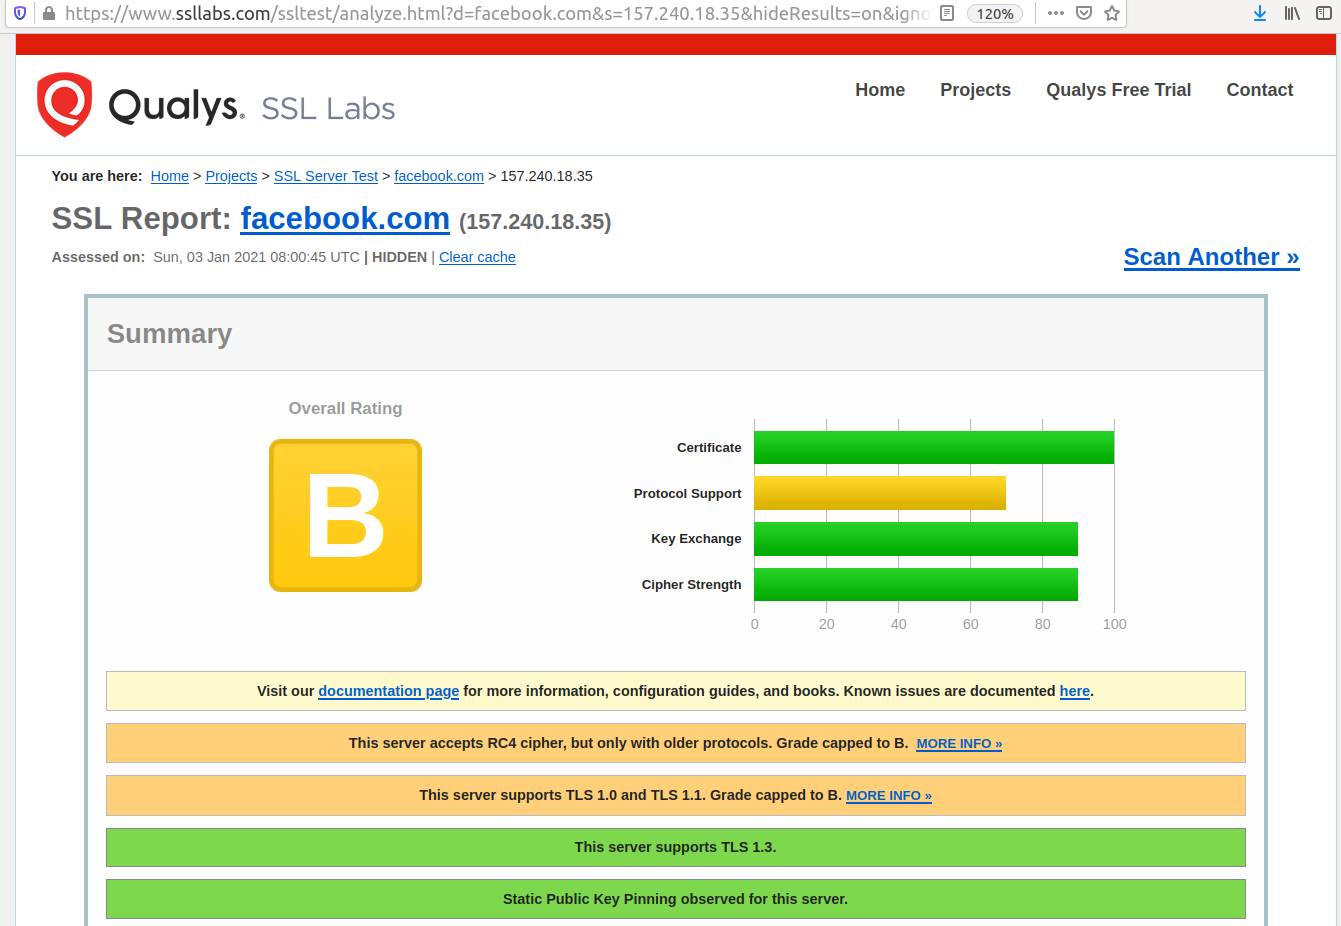
\includegraphics[width=0.8\textwidth]{chapters/12-sec/img/ssllabs.png}
  \caption{Verificarea nivelului de securitate pentru un domeniu}
  \label{fig:sec:ssllabs}
\end{figure}

Similar funcționalităților de criptare, TLS este implementat de obicei în forma unor biblioteci criptografice.
Protocoalele nesecurizate folosesc TLS pentru a obține forma lor securizată: este vorba de HTTP / HTTPS (pentru acces web), IMAP / IMAPS (pentru acces la căsuța poștală), LDAP / LDAPS (pentru interogarea directoarelor de informații).

Biblioteca OpenSSL, de care am amintit în \labelindexref{Secțiunea}{sec:sec:data:confidentiality} implementează TLS și este folosită de multe aplicații de rețea pentru a comunica securizat.
Utilitarul în linia de comandă \cmd{openssl} permite, pentru scenarii de test, construirea sau verificarea unei conexiuni securizate.
De exemplu, comanda din \labelindexref{Listing}{lst:sec:openssl-check} obține informații despre certificatul digital folosit de serverul \texttt{google.com}.

\begin{screen}[caption={Obținerea de informații despre certificatul unui domeniu},label={lst:sec:openssl-check}]
student@uso:~$ openssl s_client -connect google.com:443
CONNECTED(00000005)
depth=2 OU = GlobalSign Root CA - R2, O = GlobalSign, CN = GlobalSign
verify return:1
depth=1 C = US, O = Google Trust Services, CN = GTS CA 1O1
verify return:1
depth=0 C = US, ST = California, L = Mountain View, O = Google LLC, CN = *.google.com
verify return:1
---
Certificate chain
 0 s:C = US, ST = California, L = Mountain View, O = Google LLC, CN = *.google.com
   i:C = US, O = Google Trust Services, CN = GTS CA 1O1
 1 s:C = US, O = Google Trust Services, CN = GTS CA 1O1
   i:OU = GlobalSign Root CA - R2, O = GlobalSign, CN = GlobalSign
---
Server certificate
-----BEGIN CERTIFICATE-----
[...]
\end{screen}

\subsection{Secure Shell}
\label{sec:sec:transfer:ssh}

Transport Layer Security (TLS) permite adăugarea proprietăților de securitate pentru protocoale într-o implementare în formă de bibliotecă.
O alternativă la TLS pentru crearea unui canal sigur de comunicare este protocolul SSH (\textit{Secure Shell}).
Protocolul SSH, la fel ca TLS, oferă confidențialitate, integritate și autenticitate.
Protocolul SSH este folosind în general pentru deschiderea unei conexiuni shell sigure la distanță, pe un canal criptat.
Permite astfel administrarea unui sistem la distanță.
Este, astfel, principalul utilitar folosit în lumea Linux / Unix pentru administrarea sistemelor și este prezent pe majoritatea sistemelor de tip server.

În ciuda numelui, protocolul SSH nu este folosit numai pentru deschiderea unei sesiuni de shell sigure la distanță;
protocolul SSH creează un canal sigur de comunicare prin care se pot realiza acțiuni precum deschiderea unei sesiuni de shell la distanță, transferul de fișiere sau tunelarea unui protocol, descrise și în \labelindexref{Figura}{fig:sec:ssh-channel}.
Tunelarea unui protocol nesigur (de tip \textit{plaintext}) înseamnă că mesajele specifice acestui protocol sunt trecute prin canalul sigur de conexiune realizat de SSH.
În felul acesta SSH oferă funcționalitate similară TLS, de securizare a unui protocol.
Totuși, în TLS, protocolul în forma securizată este deja implementat, pe când în cazul SSH este nevoie de crearea canalului sigur de comunicare prin care apoi este tunelat protocolul nesigur.
Întrucât este mai simplu de folosit, preferăm folosirea protocolului securizat folosind TLS;
SSH rămâne util însă în situațiile în care nu dispunem de forma securizată a protocolului prin TLS, cum ar fi tunelarea protocolului X pentru mediul grafic în Linux, așa cum am prezentat în \labelindexref{Secțiunea}{sec:ui:window-system}.

\begin{figure}[htbp]
  \centering
  \def\svgwidth{\columnwidth}
  \includesvg[width=0.7\textwidth]{chapters/12-sec/img/ssh-channel.svg}
  \caption{Canal securizat de comunicație cu SSH}
  \label{fig:sec:ssh-channel}
\end{figure}

\begin{figure}[htbp]
  \centering
  \def\svgwidth{\columnwidth}
  \includesvg[width=0.7\textwidth]{chapters/12-sec/img/ssh-session.svg}
  \caption{Conexiune SSH}
  \label{fig:sec:ssh-session}
\end{figure}

Pentru a funcționa, protocolul SSH are nevoie de un cont de utilizator la sursă și la destinație.
Practic, realizăm un canal de comunicare sigur între două conturi de utilizator, uzual pentru deschiderea unei sesiuni de shell la distanță, ca în \labelindexref{Figura}{fig:sec:ssh-session}.
Crearea canalului se realizează numai după ce se realizează autentificarea pe contul destinație.
Autentificarea se poate realiza cu parolă sau folosind cheie publică, așa cum cum descriem în continuare.
O dată realizată autentificarea, avem un canal de comunicare prin care putem tunela comenzi (în cazul shellului), fișiere (în cazul transferului de fișiere) sau protocoale.

Pentru realizarea conexiunii SSH, la destinație trebuie să ruleze un server SSH, numit și daemon SSH.
Serverul SSH rulează uzual pe portul 22, prezența sa putând fi verificată folosind utilitarul \cmd{netstat} ca în \labelindexref{Listing}{lst:sec:ssh-netstat}.

\begin{screen}[caption={Serverul SSH},label={lst:sec:ssh-netstat}]
student@uso:~$ netstat -tln | grep 22
tcp        0      0 0.0.0.0:22              0.0.0.0:*               LISTEN
tcp6       0      0 :::22                   :::*                    LISTEN
\end{screen}

Dacă nu este prezent serverul SSH este posibil ca acesta să fie oprit sau să nu fie instalat.
Pentru instalarea și pornire / repornirea serverului SSH folosim comenzile din \labelindexref{Listing}{lst:sec:ssh-server}.
Comenzile de instalare sunt respectiv pentru sistemele Debian / Ubuntu și pentru sistemele RedHat / Fedora.

\begin{screen}[caption={Instalare și pornire server SSH},label={lst:sec:ssh-server}]
# Install SSH server on Debian / Ubuntu.
student@uso:~$ sudo apt install openssh-server

# Install SSH server on Debian / Ubuntu.
student@uso:~$ sudo dnf install openssh-server

# Restart SSH server.
student@uso:~$ sudo systemctl restart ssh
\end{screen}

Pentru deschiderea unei sesiuni shell la distanță folosim comanda \cmd{ssh} urmată de destinație: numele contului de utilizator și adresa stației destinație;
adresa stației destinație poate fi adresă IP sau nume DNS.
În \labelindexref{Listing}{lst:sec:ssh-shell} avem exemple de conexiune la distanță.
Se cere parola utilizatorului la distanță și, în cazul unei conexiuni reușite, se obține un shell care rulează la distanță cu permisiunile utilizatorului la distanță.
Pentru închiderea conexiunii, închidem procesul shell folosind comenzile \cmd{exit} sau \cmd{logout} sau combinația de taste \texttt{Ctrl+d}.

\begin{screen}[caption={Acces shell la distanță folosind SSH},label={lst:sec:ssh-shell}]
student@uso:~$ ssh malus@vmx.cs.pub.ro
malus@vmx.cs.pub.ro's password:
[...]
malus@vmx:~$ ls
extra  from-upb-to-ncsu  iOracle.git  ios-privacy-leaks  lib  prolog-data  prolog-query-work  pwn3  scripts
malus@vmx:~$ exit
logout
Connection to vmx.cs.pub.ro closed.
student@uso:~$
\end{screen}

Comanda de conexiune la distanță poate fi urmată de o altă comandă, caz în care nu se va deschide o sesiune de shell interactivă, ci se va rula acea comandă și apoi se va închide conexiunea.
În \labelindexref{Listing}{lst:sec:ssh-commands} rulăm la distanță comanda \cmd{ls} sau o comandă mai complexă pentru a afla rapid informații de pe acel sistem fără a mai fi nevoie să se deschidă o sesiune de shell interactivă.

\begin{screen}[caption={Rulare comenzi la distanță prin SSH},label={lst:sec:ssh-commands}]
student@uso:~$ ssh malus@vmx.cs.pub.ro ls
malus@vmx.cs.pub.ro's password:
extra
from-upb-to-ncsu
iOracle.git
ios-privacy-leaks
lib
prolog-data
prolog-query-work
pwn3
scripts
student@uso:~$ ssh malus@vmx.cs.pub.ro hostname
malus@vmx.cs.pub.ro's password:
vmx.cs.pub.ro
\end{screen}

Atunci când realizăm pentru prima oară o conexiune la un sistem la distanță vom primi un mesaj de avertizare că nu este cunoscută identitatea acelui sistem și suntem întrebați dacă dorim să continuăm.
În cazul în care răspundem afirmativ și continuăm, cheia publică (identitatea) acelui sistem va fi adăugată într-un fișier de configurare specific (\file{$\sim$/.ssh/known\_hosts}) și nu vom primi întrebarea mai târziu.
În \labelindexref{Listing}{lst:sec:ssh-host-check} fișierul \file{$\sim$/.ssh/known\_hosts} nu există, apoi la prima conexiune primim întrebarea și răspundem afirmativ;
fișierul \file{$\sim$/.ssh/known\_hosts} are acum intrarea corespunzătoare sistemului la distanță (cheia publică), iar la următoarea conexiune nu mai primim întrebarea, întrucât cunoaștem identitatea serverului.

\begin{screen}[caption={Verificarea identității serverului prin SSH},label={lst:sec:ssh-host-check}]
student@uso:~$ ssh malus@vmx.cs.pub.ro
The authenticity of host 'vmx.cs.pub.ro (141.85.227.139)' can't be established.
RSA key fingerprint is SHA256:CrRMD7nrflw7/KEZ4z7lksvEd8tXxkjuVXoBqsG5Vdc.
Are you sure you want to continue connecting (yes/no)? yes
Warning: Permanently added 'vmx.cs.pub.ro,141.85.227.139' (RSA) to the list of known hosts.
malus@vmx.cs.pub.ro's password:
[...]
malus@vmx:~$ logout
Connection to vmx.cs.pub.ro closed.

student@uso:~$ ssh malus@vmx.cs.pub.ro
malus@vmx.cs.pub.ro's password:
[...]
malus@vmx:~$
\end{screen}

\subsubsection{Transferul fișierelor prin SSH}
\label{sec:sec:transfer:ssh:transfer}

Pe lângă deschiderea unei conexiuni shell la distanță, protocolul SSH este folosit pentru transferul securizat de fișiere folosind utilitarul \texttt{scp} (de la \textit{secure copy}).
Comanda \cmd{scp} primește ca argument o cale locală și un nume de utilizator, adresă de stație și cale de la distanță.
În \labelindexref{Listing}{lst:sec:scp}, avem un exemplu de descărcare de fișier (\textit{download}) de la destinație (\textit{remote}) către sursă (\textit{local}) și unul de încărcare de fișier (\textit{upload}) de la sursă (\textit{local}) către destinație (\textit{remote}).

\begin{screen}[caption={Transfer de fișiere prin SSH (scp)},label={lst:sec:scp}]
student@uso:~$ mkdir malus
student@uso:~$ scp malus@vmx.cs.pub.ro:scripts/sync* malus/
malus@vmx.cs.pub.ro's password:
sync_from_ncsu_to_upb
sync.log
student@uso:~$ scp plain.txt malus@vmx.cs.pub.ro:
malus@vmx.cs.pub.ro's password:
plain.txt
student@uso:~$ scp malus@vmx.cs.pub.ro:scripts/sync.log .
malus@vmx.cs.pub.ro's password:
sync.log
student@uso:~$ ls sync.log
sync.log
student@uso:~$ scp -r malus@vmx.cs.pub.ro:scripts .
malus@vmx.cs.pub.ro's password:
.sync_from_ncsu_to_upb.un~
sync.log
sync_from_ncsu_to_upb
\end{screen}

De multe ori în cazul descărcării unui fișier destinația este \file{.} (punct) adică realizăm transferul de la distanță în directorul curent, ca în liniile 9-13 din \labelindexref{Listing}{lst:sec:scp}.
Similar comenzii \cmd{cp}, putem folosi comanda \cmd{scp} pentru a transfera recursiv o ierarhie de directoare și fișiere ca în liniile 14-18 din \labelindexref{Listing}{lst:sec:scp}.

\subsubsection{Autentificarea cu cheie publică prin SSH}
\label{sec:sec:transfer:ssh:pub-auth}

În mod implicit, realizarea unei conexiuni SSH necesită introducerea parolei contului utilizatorului de la distanță.
Așa cum am precizat în \labelindexref{Secțiunea}{sec:sec:auth:password}, autentificarea cu parole poate fi problematică dacă parolele nu sunt gestionate corespunzător.
De aceea, în multe situații dorim să înlocuim folosirea autentificării cu parole cu altă formă de autentificare pentru SSH.

O formă alternativă de autentificare pentru SSH este autentificarea cu cheie publică.
Această autentificare presupune existența unei perechi cheie publică / cheie privată, ca în cazul semnăturilor digitale, descrise în \labelindexref{Secțiunea}{sec:sec:transfer:sign}.
Cheia privată este deținută de utilizator local.
Cheia publică trebuie să fie adăugată în contul utilizatorului de la distanță.
În momentul în care se realizează autentificarea, protocolul SSH folosește cheia privată a utilizatorului local pentru a semna un mesaj.
Mesajul și semnătură sunt transmise la distanță, unde se folosește cheia publică deja adăugată în contul utilizatorului de la distanță pentru a verifica mesajul.
Autentificarea reușește dacă utilizatorul de la distanță deține cheia publică a utilizatorului local.
În acel moment canalul SSH este creat.

Astfel, pentru realizarea unei conexiuni SSH cu autentificare prin cheie publică, trebuie urmați pașii următori:
\begin{enumerate}
  \item Se generează perechea cheie privată / cheie publică în contul utilizatorului local.
  \item Se adaugă cheia publică în contul utilizatorului de la distanță.
  \item Se folosește cheia privată din contul utilizatorului local pentru crearea unei conexiuni SSH.
    Aceasta se va realiza fără parolă.
\end{enumerate}

În mod obișnuit, generarea perechii cheie privată / cheie publică se realizează o singură dată.
Apoi cheia publică se adaugă în conturile de utilizator de la distanță pentru a permite autentificarea fără parolă.
Cheia publică SSH este configurată și în alte servicii care se bazează pe SSH precum GitHub.

În Linux, pentru generarea unei perechi cheie privată / cheie publică se folosește utilitarul \cmd{ssh-keygen}, ca în \labelindexref{Listing}{lst:sec:ssh-keygen}.
Așa cum se afișează și la promptul rulării \cmd{ssh-keygen}, în mod implicit cheile sunt generate în directorul \file{$\sim$/.ssh/}: cheia privată este în fișierul \file{$\sim$/.ssh/id\_rsa}, iar cheia publică este în fișierul \file{$\sim$/.ssh/id\_rsa.pub}.
Întrucât deja existau cheile implicite, în \labelindexref{Listing}{lst:sec:ssh-keygen}, am generat o nouă pereche cheie privată / cheie publică în fișierele \file{$\sim$/.ssh/new\_id}, respectiv \file{$\sim$/.ssh/new\_id.pub}.

\begin{screen}[caption={Generarea unei perechi cheie privată / cheie publică SSH},label={lst:sec:ssh-keygen}]
student@uso:~$ ls ~/.ssh/
id_rsa  id_rsa.pub  known_hosts
student@uso:~$ ssh-keygen
Generating public/private rsa key pair.
Enter file in which to save the key (/home/student/.ssh/id_rsa): /home/student/.ssh/new_id 
Enter passphrase (empty for no passphrase):
Enter same passphrase again:
[...]
student@uso:~$ ls ~/.ssh/
id_rsa  id_rsa.pub  known_hosts  new_id  new_id.pub
\end{screen}

Adăugarea cheii publice în contul utilizatorului de la distanță se realizează în fișierul \file{$\sim$/.ssh/authorized\_keys}.
Acest fișier conține toate cheile publice pentru care se permite autentificare (cu cheie publică) la contul utilizatorului.
Adăugarea se face prin copierea conținutului cheii publice în cadrul fișierului.
Sau se poate folosi utilitarul \cmd{ssh-copy-id} pentru a copia cheia publică a utilizatorului curent în contul utilizatorului de la distanță, ca în \labelindexref{Listing}{lst:sec:ssh-copy-id}.

\begin{screen}[caption={Copierea cheii publice la distanță},label={lst:sec:ssh-copy-id}]
student@uso:~$ ssh-copy-id malus@vmx.cs.pub.ro
/usr/bin/ssh-copy-id: INFO: Source of key(s) to be installed: "/home/student/.ssh/id_rsa.pub"
/usr/bin/ssh-copy-id: INFO: attempting to log in with the new key(s), to filter out any that are already installed
/usr/bin/ssh-copy-id: INFO: 1 key(s) remain to be installed -- if you are prompted now it is to install the new keys
malus@vmx.cs.pub.ro's password: 

Number of key(s) added: 1

Now try logging into the machine, with:   "ssh 'malus@vmx.cs.pub.ro'"
and check to make sure that only the key(s) you wanted were added.
\end{screen}

În urma copierii cheii publice în contul utilizatorului de la distanță, se poate realiza autentificarea fără parolă, ca în \labelindexref{Listing}{lst:sec:ssh-pub-auth}, liniile 1-4.
Dacă dorim să folosim o anumită cheie privată (perechea cheii publice) pentru autentificare, transmite opțiunea \texttt{-i} (de la \textit{identity}) comenzii \cmd{ssh} (sau \cmd{ssh-copy-id}, ca în \labelindexref{Listing}{lst:sec:ssh-pub-auth}, liniile 6-21;
opțiunea este urmată de calea către fișierul ce conține cheia privată.

\begin{screen}[caption={Autentificarea SSH cu cheie publică},label={lst:sec:ssh-pub-auth}]
student@uso:~$ ssh malus@vmx.cs.pub.ro
[...]
malus@vmx:~$ logout
Connection to vmx.cs.pub.ro closed.

student@uso:~$ ssh -i ~/.ssh/new_id malus@vmx.cs.pub.ro
malus@vmx.cs.pub.ro's password:

student@uso:~$ ssh-copy-id -i ~/.ssh/new_id.pub malus@vmx.cs.pub.ro
/usr/bin/ssh-copy-id: INFO: Source of key(s) to be installed: "/home/student/.ssh/new_id.pub"
/usr/bin/ssh-copy-id: INFO: attempting to log in with the new key(s), to filter out any that are already installed
/usr/bin/ssh-copy-id: INFO: 1 key(s) remain to be installed -- if you are prompted now it is to install the new keys

Number of key(s) added: 1

Now try logging into the machine, with:   "ssh 'malus@vmx.cs.pub.ro'"
and check to make sure that only the key(s) you wanted were added.

student@uso:~$ ssh -i ~/.ssh/new_id malus@vmx.cs.pub.ro
[...]
malus@vmx:~$
\end{screen}

\subsubsection{SSH în Windows}
\label{sec:sec:transfer:ssh:windows}

Deși specific lumii Linux / Unix, protocolul SSH este folosit și în lumea Windows.
În general, folosim SSH în Windows în aplicații client, pentru a ne conecta la sisteme Linux / Unix la distanță.
Totuși, se poate instala un server SSH și în Windows, de exemplu Bitvise SSH Server\footnote{\url{https://www.bitvise.com/ssh-server}}.

Cele mai întâlnite aplicații de tip client SSH pe Window sunt PuTTY\footnote{\url{https://www.putty.org/}}, WinSCP\footnote{\url{https://winscp.net/eng/download.php}} și Bitvise SSH Client\footnote{\url{https://www.bitvise.com/ssh-client}}.

PuTTY (în \labelindexref{Figura}{fig:sec:putty}) este folosit pentru realizarea unei conexiuni SSH la distanță.
Conține și utilitare asociate pentru generarea de perechi cheie privată / cheie publică (PuTTYgen) și pentru transferul de informații la distanță (PSCP).

WinSCP (în \labelindexref{Figura}{fig:sec:winscp}) oferă o interfață de tip \textit{commander} pentru transferul de fișiere prin SSH.

\begin{figure}[!htbp]
  \centering
  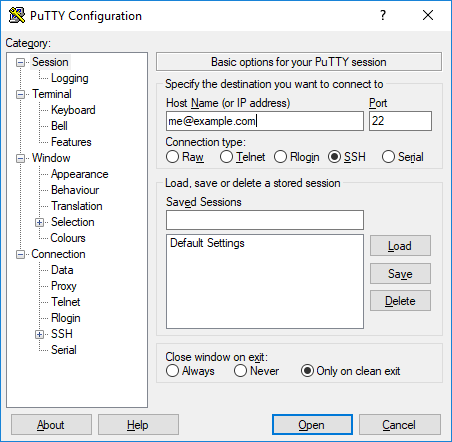
\includegraphics[width=0.7\textwidth]{chapters/12-sec/img/putty.png}
  \caption{PuTTY}
  \label{fig:sec:putty}
\end{figure}

\begin{figure}[!htbp]
  \centering
  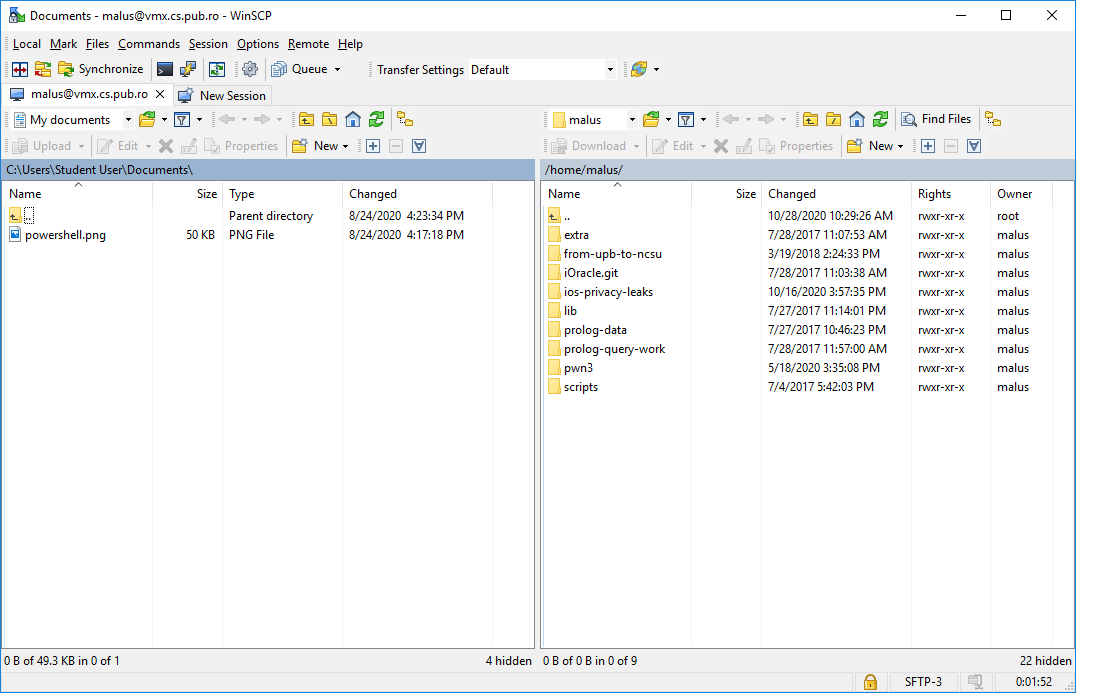
\includegraphics[width=0.7\textwidth]{chapters/12-sec/img/winscp.png}
  \caption{WinSCP}
  \label{fig:sec:winscp}
\end{figure}

\section{Securitatea proceselor}
\label{sec:sec:process}

Un utilizator folosește resursele unui sistem (hardware, fișiere, servicii) cu ajutorul proceselor.
La fel, un atacator care dorește să abuzeze un sistem (să-l controleze, să fure informații sau să-i afecteze funcționarea) va dori capturarea unor procese.
Un mod direct pentru capturarea unui proces este ca atacatorul să obțină credențialele de acces și să impersoneze un utilizator valid în sistem, obținând permisiunile acestuia, așa cum am descris în \labelindexref{Secțiunea}{sec:sec:auth}.
Un alt mod este exploatând vulnerabilități ale procesului și capturând astfel procesul.
Alt mod este păcălind utilizatorul să instaleze aplicații create de atacator care să pornească procese care să abuzeze sistemele.
Aceste aplicații malițioase sunt numite \textbf{malware}: virușii, troienii, viermii (\textit{worms}), spyware sunt exemple de malware.

În oricare dintre variantele de mai sus, sistemul de operare trebuie să aibă în vedere măsuri preventive și măsuri reactive pentru protejarea proceselor.

Măsurile preventive vizează împiedicarea unui atacator să poată ajunge la procese din sistem.
Aceste măsuri pot fi:

\begin{itemize}
  \item securitatea accesului la sistem (descrisă în \labelindexref{Secțiunea}{sec:sec:auth})
  \item tehnici specializate (precum protejarea memoriei) care să împiedice exploatarea vulnerabilităților
  \item verificarea aplicațiilor instalate (folosind rezumate / sume de control) și verificarea sursei de proveniență.
    Aceasta este foarte importantă mai ales în cazul dispozitivelor mobile unde magazinele online de aplicații (\textit{online application stores}) precum Apple AppStore sau Google Play stochează foarte multe aplicații.
\end{itemize}

Măsurile reactive presupun că atacul s-a produs sau se va produce și vizează limitarea daunelor produse de un atac.
Astfel de măsuri sunt: plasarea procesului contaminat în carantină, investigația atacului și depistarea problemei, actualizarea aplicației vulnerabile (\textit{update}, \textit{patching}) sau înlăturarea aplicației vulnerabile.

Măsurile reactive trebuie să fie luate cât mai repede după producerea unui atac pentru a limita daunele.
De aceea, este importantă \textbf{monitorizarea proceselor} și resurselor unui sistem.
Un utilizator tehnic sau un administrator de sistem sau de rețea va folosi suite de aplicații specifice pentru monitorizare și va depista comportamente anormale care pot fi efectele unui atac și va reacționa rapid.
În absența monitorizării, un atacator va avea mai mult timp pentru a obține beneficii în urma atacului sau va putea extinde atacul la alte sisteme sau resurse.
Monitorizarea are rolul de a depista atât atacurile, cât și abuzul de resurse sau comportamente neobișnuite datorate unei utilizări necorespunzătoare (dar neintenționat abuzive) a sistemului.
De exemplu, sistemele de tip antivirus monitorizează periodic sistemul de fișiere pentru a detecta prezența fișierelor infectate.
Utilitare precum Fail2ban\footnote{\url{https://www.fail2ban.org/wiki/index.php/Main\_Page}} monitorizează fișiere de tip jurnal pentru a detecta și a bloca încercări de acces nevalid în sistem.
Sisteme complexe precum Nagios\footnote{\url{https://www.nagios.org/}} monitorizează infrastructura IT a unei organizații: rețea, aplicații, resurse hardware.

Pentru prevenirea daunelor produse de un proces compromis, este esențială respectarea principiului celui mai mic privilegiu, descris în \labelindexref{Secțiunea}{sec:sec:fundamentals:principles}.
Acesta presupune ca un proces să aibă acces doar la resursele de care are nevoie: fișiere, interacțiune cu alte procese, resurse hardware.

Un prim mod de implementarea a principiului celui mai mic privilegiu îl reprezintă permisiunile de acces la sistemul de fișiere.
Un proces va putea accesa doar acele fișiere la care are acces utilizatorul de care aparține procesul.
Astfel, un proces al unui utilizator neprivilegiat va putea scrie doar în directorul home propriu, va putea doar citi fișierul \file{/etc/passwd} și nu va avea nici o formă de acces la fișierul \file{/etc/shadow}.

O măsură suplimentară este folosirea de mecanisme de jailing de tipul chroot, așa cum am descris în \labelindexref{Secțiunea}{sec:sec:data:fs}.
Cu un astfel de mecanism, un proces va putea accesa doar fișierele dintr-o parte a ierarhiei sistemului de fișiere.

Mecanismele de tipul chroot sunt mecanisme de \textbf{izolare a procesului}.
Cu ajutorul chroot izolăm accesul procesului la sistemul de fișiere.
Pentru a extinde izolarea și în alte zone (comunicarea cu alte procese, accesul la rețea, accesul la hardware), putem folosi \textbf{sandboxing}.
Sandboxing presupune crearea unor reguli de acces la resurse și atașarea acelor reguli la un proces;
procesul va putea accesa doar resursele permise în acele reguli.
Sandboxingul este implementat în sistemele de operare de pe dispozitivele mobile (Android, iOS) pentru a limita potențialele daune create de aplicații instalate de un utilizator pe dispozitivul mobil.

O formă extinsă de izolare este \textbf{folosirea containerelor sau mașinilor virtuale}, descrise în \labelindexref{Capitolul}{ch:vm}.
Containerele oferă reguli complexe de izolare a unei aplicații sau a unui set de aplicații, extinzând astfel mecanismul de sandboxing.
Mașinile virtuale adaugă, față de containere, partiționarea resurselor hardware și izolarea inclusiv a sistemului de operare al mașinii virtuale;
în cazul unui sistem de operare compromis, doar mașina virtuală respectivă va fi afectată.

Prezența metodelor de izolare duce la diminuarea daunelor produse de un potențial atac.
Dar izolarea unui proces limitează plaja de acțiuni a acestuia.
Este posibil ca un proces să aibă nevoie, la un moment dat, de o acțiune privilegiată care nu poate fi realizată conform regulilor de izolare.
Pentru această acțiuni este nevoie de escaladarea nivelului de privilegiu (\textit{privilege escalation}), adică obținerea (temporară) de privilegii care să permită acțiunea.

În Linux, forma clasică de escaladare a privilegiilor este marcarea unui executabil cu bitul \textit{set-user-ID-on-execution} (numit și \textit{setuid}).
O formă configurabilă de escaladare de privilegii este cu ajutorul utilitarului \cmd{sudo}.
Am detaliat bitul setuid și utilitarul \cmd{sudo} în \labelindexref{Secțiunea}{sec:user:altroot}.

Întrucât procesele sunt modul de utilizare a sistemului și accesarea a resurselor acestuia, trebuie să avem în vedere securitatea acestora prin măsuri preventive și măsuri reactive.
Este important sa avem grijă ce aplicații instalăm pe sistemele și dispozitivele noastre și să folosim aplicații care monitorizează funcționarea sistemului și folosirea resurselor acestuia.

\section{Sumar}
\label{sec:sec:summary}

Un sistem este sigur dacă este folosit așa cum a fost proiectat.
Întrucât este cvasi-imposibil să acoperim toate cazurile în care un sistem poate fi folosit, nu putem spune că un sistem este perfect sigur.
Spunem că securitatea este un proces, nu o finalitate.

Un atacator poate urmări să controleze un sistem, să fure informații sau să abuzeze resurse.
Un apărător urmărește să prevină existența atacurilor sau reacționeze cât mai rapid pentru a limita daunele unui atac.
Un apărător va urmări să asigure confidențialitatea datelor, integritate datelor, disponibilitatea serviciilor și protejarea vieții private (\textit{privacy}).

Pentru protejarea unui sistem, există principii de securitate pe care utilizatorii și organizațiile să le urmeze: cel mai mic privilegiu, securitate în adâncime, separarea mecanismului de politică, proiectare modulară.

Un utilizator sau administrator se va preocupa de securitatea accesului (cine are acces la sistem și la ce resurse), securitatea transferului (cum se transmit informațiile în Internet) si securitatea aplicațiilor (o aplicație să fie protejată de atacuri sau, dacă este atacată, să nu afecteze alte aplicații).

Există protocoale, algoritmi, tehnologii și aplicații pentru creșterea securității unui sistem.
Un utilizator / administrator va fi în permanență informat, va aloca resurse și va depune efort constant pentru a garanta un nivel optim de securitate.
